% Standalone article: bibliography and all vector figures are embedded.
% Compile with latexmk -pdf; requires Biber and standard TeX packages.
\begin{filecontents*}[overwrite]{paper3_references.bib}
@article{Mao2012MDP,
 author={Mao, Hua and Chen, Yingke and Jaeger, Manfred and Nielsen, Thomas D. and Larsen, Kim G. and Nielsen, Brian},
 title={Learning {Markov Decision Processes} for Model Checking},
 journal={Electronic Proceedings in Theoretical Computer Science}, volume={103}, pages={49--63}, year={2012},
 doi={10.4204/EPTCS.103.6}, eprint={1212.3873}, eprinttype={arxiv}
}
@inproceedings{MaoJaeger2012,
 author={Mao, Hua and Jaeger, Manfred}, title={Learning and Model-Checking Networks of {I/O} Automata},
 booktitle={Proceedings of the Asian Conference on Machine Learning}, series={Proceedings of Machine Learning Research}, volume={25}, pages={285--300}, year={2012},
 url={https://proceedings.mlr.press/v25/mao12.html}
}
@misc{Tappler2019,
 author={Tappler, Martin and Aichernig, Bernhard K. and Bacci, Giovanni and Eichlseder, Maria and Larsen, Kim G.},
 title={{L*}-Based Learning of {Markov Decision Processes} (Extended Version)}, year={2019},
 eprint={1906.12239}, eprinttype={arxiv}, doi={10.48550/arXiv.1906.12239}
}
@misc{Shijubo2023,
 author={Shijubo, Junya and Waga, Masaki and Suenaga, Kohei},
 title={Probabilistic Black-Box Checking via Active {MDP} Learning}, year={2023},
 eprint={2308.07930}, eprinttype={arxiv}, doi={10.48550/arXiv.2308.07930}, note={Preprint accepted to EMSOFT 2023}
}
@article{Baum1970,
 author={Baum, Leonard E. and Petrie, Ted and Soules, George and Weiss, Norman},
 title={A Maximization Technique Occurring in the Statistical Analysis of Probabilistic Functions of {Markov} Chains},
 journal={The Annals of Mathematical Statistics}, volume={41}, number={1}, pages={164--171}, year={1970}, doi={10.1214/aoms/1177697196}
}
@article{Hsu2012,
 author={Hsu, Daniel and Kakade, Sham M. and Zhang, Tong},
 title={A Spectral Algorithm for Learning Hidden {Markov} Models},
 journal={Journal of Computer and System Sciences}, volume={78}, number={5}, pages={1460--1480}, year={2012},
 eprint={0811.4413}, eprinttype={arxiv}
}
@article{Barnett2015,
 author={Barnett, Nix and Crutchfield, James P.},
 title={Computational Mechanics of Input--Output Processes: Structured Transformations and the $\epsilon$-Transducer},
 journal={Journal of Statistical Physics}, volume={161}, number={2}, pages={404--451}, year={2015},
 doi={10.1007/s10955-015-1327-5}, eprint={1412.2690}, eprinttype={arxiv}
}
@article{Bengio1995,
 author={Bengio, Yoshua and Frasconi, Paolo},
 title={Diffusion of Context and Credit Information in {Markovian} Models},
 journal={Journal of Artificial Intelligence Research}, volume={3}, pages={249--270}, year={1995},
 eprint={cs/9510101}, eprinttype={arxiv}
}
@article{Cawley2010,
 author={Cawley, Gavin C. and Talbot, Nicola L. C.},
 title={On Over-fitting in Model Selection and Subsequent Selection Bias in Performance Evaluation},
 journal={Journal of Machine Learning Research}, volume={11}, pages={2079--2107}, year={2010},
 url={https://www.jmlr.org/papers/v11/cawley10a.html}
}
@misc{Dwork2015,
 author={Dwork, Cynthia and Feldman, Vitaly and Hardt, Moritz and Pitassi, Toniann and Reingold, Omer and Roth, Aaron},
 title={Generalization in Adaptive Data Analysis and Holdout Reuse}, year={2015},
 eprint={1506.02629}, eprinttype={arxiv}, doi={10.48550/arXiv.1506.02629}
}
@misc{Rubenstein2017,
 author={Rubenstein, Paul K. and Weichwald, Sebastian and Bongers, Stephan and Mooij, Joris M. and Janzing, Dominik and Grosse-Wentrup, Moritz and Sch{\"o}lkopf, Bernhard},
 title={Causal Consistency of Structural Equation Models}, year={2017},
 eprint={1707.00819}, eprinttype={arxiv}, note={Proceedings of UAI 2017}
}
@article{Baez2018,
 author={Baez, John C. and Courser, Kenny}, title={Coarse-Graining Open {Markov} Processes},
 journal={Theory and Applications of Categories}, volume={33}, number={39}, pages={1223--1268}, year={2018},
 eprint={1710.11343}, eprinttype={arxiv}
}
@article{Gebler2013,
 author={Gebler, Daniel and Tini, Simone}, title={Compositionality of Approximate Bisimulation for Probabilistic Systems},
 journal={Electronic Proceedings in Theoretical Computer Science}, volume={120}, pages={32--46}, year={2013},
 doi={10.4204/EPTCS.120.4}, eprint={1307.7442}, eprinttype={arxiv}
}
@misc{vanRooyen2014,
 author={van Rooyen, Brendan and Williamson, Robert C.}, title={{Le Cam} meets {LeCun}: Deficiency and Generic Feature Learning},
 year={2014}, eprint={1402.4884}, eprinttype={arxiv}, doi={10.48550/arXiv.1402.4884}
}
@online{AALpySource,
 author={{DES-Lab}}, title={{AALpy}: Stochastic Passive Learning Source Code},
 url={https://github.com/DES-Lab/AALpy/tree/master/aalpy/learning_algs/stochastic_passive},
 urldate={2026-09-29}, note={Alergia.py and CompatibilityChecker.py. Methodological reference; the study executed a local adaptation, not the upstream package}
}
@misc{RodgersPaper2,
 author={Rodgers, Jeremy}, title={Relational Boundaries and Awareness Localization: Robustness, Composition, and Identification Limits},
 date={2026-09-29}, version={1.0}, publisher={Zenodo}, doi={10.5281/zenodo.23075822},
 note={Companion preprint, Paper 2; supplied source snapshot retained in the present supplement}
}

@misc{RodgersSPC2,
 author={Rodgers, Jeremy},
 title={Shadow Theory and Consciousness: Awareness, Perspectival Realization, and the Source-to-Experience Problem},
 date={2026-09-20}, version={2}, publisher={Zenodo},
 doi={10.5281/zenodo.22853774},
 url={https://www.everythingequation.com/consciousness/monograph},
 note={Publication edition}
}
@misc{RodgersPaper4,
 author={Rodgers, Jeremy},
 title={Identifying Binary Realizations from Intervention Laws: Certificates, Recoding Obstructions, and a Bounded {SPC-2}/{IIT} Comparison},
 date={2026-09-30}, version={1.1-RC1}, publisher={Zenodo},
 doi={10.5281/zenodo.23075828},
 note={Companion preprint, Paper 4}
}

@misc{RodgersEvidence,
 author={Rodgers, Jeremy}, title={Paper 3 Evidence, Attribution, and Claim Freeze},
 date={2026-09-29}, note={Versioned source snapshot containing RRI and OII-1--4 evidence, protocols, scores and claim ledgers. Preserved unchanged in the manuscript supplement; archive hash in SOURCE\_INPUT\_MANIFEST.json}
}

@inproceedings{Littman2001PSR,
 author={Littman, Michael L. and Sutton, Richard S. and Singh, Satinder},
 title={Predictive Representations of State},
 booktitle={Advances in Neural Information Processing Systems}, volume={14},year={2001},
 url={https://proceedings.neurips.cc/paper_files/paper/2001/file/1e4d36177d71bbb3558e43af9577d70e-Paper.pdf},
 note={NIPS 2001; author list verified against the paper PDF}}
@inproceedings{Singh2004PSR,
 author={Singh, Satinder and James, Michael R. and Rudary, Matthew R.},
 title={Predictive State Representations: A New Theory for Modeling Dynamical Systems},
 booktitle={Proceedings of the Twentieth Conference on Uncertainty in Artificial Intelligence},
 year={2004},pages={512--519},eprint={1207.4167},eprinttype={arxiv},
 note={UAI 2004; author-deposited repository version uploaded in 2012}}
@misc{Boots2009PSR,
 author={Boots, Byron and Siddiqi, Sajid M. and Gordon, Geoffrey J.},
 title={Closing the Learning-Planning Loop with Predictive State Representations},
 year={2009},eprint={0912.2385},eprinttype={arxiv},
 note={Inspected author-deposited preprint, version 1}}
\end{filecontents*}
% Modular entry point. The separately supplied FINAL.tex inlines this source.

% BEGIN preamble.tex
\documentclass[11pt,a4paper]{article}
\usepackage[T1]{fontenc}
\usepackage[utf8]{inputenc}
\usepackage{amsmath,amsthm,mathtools}
\usepackage{newtxtext,newtxmath}
\usepackage[margin=25mm,headheight=14pt]{geometry}
\usepackage{microtype}
\usepackage{booktabs,tabularx,longtable,array,multirow}
\usepackage{graphicx,tikz,pgfplots}
\usetikzlibrary{arrows.meta,positioning,calc,fit}
\pgfplotsset{compat=1.18}
\usepackage{enumitem}
\usepackage{float,placeins}
\usepackage[font=small,labelfont=bf]{caption}
\usepackage{csquotes}
\usepackage[backend=biber,style=numeric,sorting=nyt,maxbibnames=9,giveninits=true,doi=true,isbn=false,url=true]{biblatex}
\addbibresource{paper3_references.bib}
\usepackage{xurl}
\usepackage[hidelinks]{hyperref}
\usepackage[nameinlink,noabbrev]{cleveref}
\usepackage{fancyhdr}
\pagestyle{fancy}\fancyhf{}
\fancyhead[L]{\small Learning Effective Stochastic Interfaces}
\fancyhead[R]{\small Jeremy Rodgers}
\fancyfoot[C]{\thepage}
\setlength{\parindent}{1.2em}
\setlength{\parskip}{.25em}
\setlength{\emergencystretch}{2em}
\setcounter{topnumber}{3}\setcounter{bottomnumber}{2}\setcounter{totalnumber}{4}
\renewcommand{\topfraction}{.92}\renewcommand{\bottomfraction}{.85}\renewcommand{\textfraction}{.08}\renewcommand{\floatpagefraction}{.78}
\newtheorem{proposition}{Proposition}[section]
\newtheorem{lemma}[proposition]{Lemma}
\theoremstyle{definition}\newtheorem{definition}[proposition]{Definition}
\theoremstyle{remark}\newtheorem{remark}[proposition]{Remark}
\DeclareMathOperator{\TV}{TV}\DeclareMathOperator{\Law}{Law}\DeclareMathOperator{\rad}{rad}\DeclareMathOperator*{\argmin}{arg\,min}
\newcommand{\E}{\mathcal E}\newcommand{\HH}{\mathcal H}\newcommand{\BB}{\mathcal B}\newcommand{\one}{\mathbf 1}
\newcommand{\RRC}{\textsf{RRC}}\newcommand{\RJC}{\textsf{RJC}}
\newcommand{\iid}{i.i.d.}
\newcolumntype{Y}{>{\raggedright\arraybackslash}X}
\hypersetup{pdftitle={Learning Effective Interfaces from Opaque Stochastic Systems: Capacity, Selection, and Validation Limits},pdfauthor={Jeremy Rodgers},pdfsubject={Finite stochastic interface learning and validation limits},pdfkeywords={system identification, probabilistic automata, hidden Markov models, interface learning, model selection}}

% END preamble.tex


% BEGIN tables/numeric_macros.tex
% Generated from frozen evidence; see code/generate_tables.py
\newcommand{\SuiteFixtures}{48}
\newcommand{\SuiteSlots}{1,152}
\newcommand{\UniqueSlots}{1,140}
\newcommand{\CalibrationOverlapSlots}{79}
\newcommand{\CalibrationOverlapUnique}{74}
\newcommand{\SharedCalls}{442,368}
\newcommand{\SharedResets}{55,296}
\newcommand{\TrainCalls}{7,680}
\newcommand{\CalibrationCalls}{1,536}
\newcommand{\EvidenceCalls}{9,216}
\newcommand{\RPass}{1063}
\newcommand{\SPass}{1063}
\newcommand{\PPass}{970}
\newcommand{\OPass}{869}
\newcommand{\BPass}{1053}
\newcommand{\RMean}{0.054913}
\newcommand{\SMean}{0.054918}
\newcommand{\PMean}{0.099072}
\newcommand{\OMean}{0.152015}
\newcommand{\BMean}{0.064684}

% END tables/numeric_macros.tex

\begin{document}

% BEGIN sections/00_front.tex
\title{Learning Effective Interfaces from Opaque Stochastic Systems:\\Capacity, Selection, and Validation Limits}
\author{Jeremy Rodgers\\\small Independent Researcher\\\small Website: \href{https://www.everythingequation.com}{everythingequation.com}\\\small DOI: \href{https://doi.org/10.5281/zenodo.23075824}{10.5281/zenodo.23075824}}
\date{29 September 2026\\\small Revised preprint v2: post-hoc optimization sensitivity included}
\maketitle
\begin{abstract}
An effective stochastic interface can be precisely specified without being reliably recovered from restricted observations. We study this gap in finite software investigations, culminating in a same-evidence comparison on 48 opaque systems. A portfolio of probabilistic automata and controlled hidden-state models passes 1,063 of 1,152 registered complete-law tests at total-variation allowance 0.15, compared with 970 for a passive tree control and 869 for a minimax tree bank. A prespecified secondary portfolio without the bespoke group-aware candidates reproduces the broad gain. An elementary post-reveal capacity check rules out insufficient architectural expressiveness: all targets fit the general 16-state instrument family. Under the original fitting budget, however, only 39 fixtures receive an individually passing produced candidate and 37 receive one from calibration selection. A separate post-hoc sensitivity analysis targets the 11 failures, using six starts per latent size and at most 600 rather than 60 updates on unchanged public data. The expanded portfolio selects a passing model on five failures and contains one on seven. Four passing controls retain their original selections. Thus the original candidate-production gap is materially budget-sensitive, while selection and residual fitting failures persist. Exact conditional diagnostics show that the challenge regressions involve mixing preparation-dependent responses rather than simple loss of the observed challenge. Paired fixture summaries, full-law re-evaluation, and retrospective policy-equivalence audits support transparent reporting without altering primary scores. The study separates capacity, finite-budget production, selection and validation coverage; its same-author, outcome-selected sensitivity is not an independently authored benchmark or a new primary result.
\end{abstract}
\noindent\textbf{Keywords:} stochastic system identification; probabilistic automata; hidden-state models; model selection; optimization sensitivity; interface abstraction.

% END sections/00_front.tex


% BEGIN sections/01_introduction.tex
\section{Question and contributions}\label{sec:intro}\label{p3:c01}
Replacing a subsystem by a smaller model is useful only insofar as the replacement preserves behavior that later interactions can expose. A queue can appear empty while retaining a delayed message; a service can return the correct first answer while forgetting that its only resource has been spent; two outputs can have correct marginal distributions and an incorrect joint law. These are reasons to evaluate an interface through complete interaction histories rather than isolated predictions. They do not, however, prescribe an algorithm that will learn such an interface from a finite observation budget.

The distinction between a specification of adequacy and successful identification is familiar in probabilistic verification and system identification. Reactive automata learning already combines observed input--output behavior with formal model analysis \cite{Mao2012MDP,MaoJaeger2012}. Our contribution is not to claim this distinction as a new general principle. We give a source-preserved sequence of computational tests in which progressively plausible repairs can be compared, and failures can sometimes be localized more sharply than by a single predictive score.

The motivating contract comes from a companion theoretical paper \cite{RodgersPaper2}. Its robust joint-candidate diagnostics (\RJC) distinguish joint information, native execution and resource-relative simulation; its robust relational-composition analysis (\RRC) specifies conditions for substituting an effective process in a matching causal context. The broader psychophysical programme is developed in the monograph \cite{RodgersSPC2}. The present paper imports only the operational adequacy obligations. An adequate predictive model and a certified marked source quotient are different objects; the companion's awareness interpretation is not part of this study.

We examine four opaque-interface identification stages, denoted OII-1 through OII-4, after a known-model implementation-conformance stage, RRI. The stages have different cohorts, acquisition allocations and candidate families. They are not replications of one unchanged design, and their scores must not be read as a controlled longitudinal learning curve. The final OII-4 study is the principal matched endpoint: all eight reported methods use one common fitting/calibration tape per fixture and the same scored laws. Earlier stages supply the failure-driven development and the analytical diagnoses.

Three findings organize the paper. First, the tested standard automata/hidden-state portfolio improves several aggregate metrics over the tree controls on the final suite, but not every mechanism family. Second, adding two group-aware automata candidates is not needed to reproduce the broad improvement: the prespecified secondary portfolio without them has essentially identical outcomes. Third, an elementary post-reveal capacity check rules out literal architectural insufficiency for the final targets, while the original fitting procedure still misses adequate candidates. A new, separately labeled optimization-sensitivity analysis shows that increased fitting effort repairs a material part of that gap. It also exposes continuing selection failures and more specific challenge-response errors. These findings separate architectural existence from finite-budget candidate production and public-data selection.

The unit of evidence is important. A complete-law test slot is not an independent Bernoulli trial. A fresh generator instance is not necessarily tested under an unseen policy specification. Exact oracle scores are withheld from the learner, but some evaluation specifications also occur in public calibration. We report those overlaps, the original primary and secondary method designations, the severe regressions, and the preserved pre-score repairs. These qualifications delimit the result; they are not reasons to hide the study's useful finite conclusions.

All primary performance values derive from the frozen evidence package \cite{RodgersEvidence}. Manuscript assembly corrected the description of the hidden-state fitting limit: the original code uses at most 60 iterations with early stopping. The subsequent methodological audit independently reconstructed the OII-4 law evaluations from saved sources and parameters and extended the retrospective context audit from literal descriptions to complete finite policy behavior. Those audit stages did not refit learners. The present revision adds 360 separately stored post-hoc fits after a local protocol lock, using the existing public tapes and without changing any original model, primary score or weight. The 11 failures were selected using known original outcomes, so this sensitivity is not a fresh blind experiment. Its own candidate selections were committed before the new core evaluations.


% BEGIN figures/pipeline.tex
\begin{figure}[tbp]
\centering
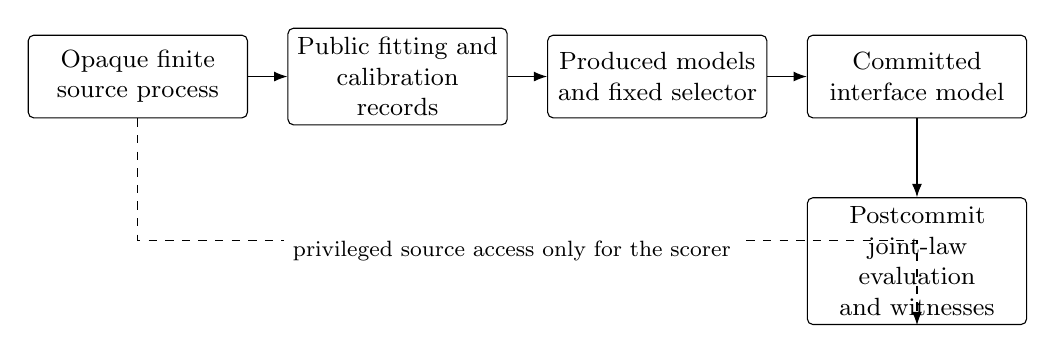
\begin{tikzpicture}[>=Latex,box/.style={draw,rounded corners=2pt,align=center,text width=2.55cm,minimum height=1.05cm,font=\small},node distance=5mm]
\node[box] (system) {Opaque finite\\source process};
\node[box,right=of system] (tape) {Public fitting and\\calibration records};
\node[box,right=of tape] (bank) {Produced models\\and fixed selector};
\node[box,right=of bank] (model) {Committed\\interface model};
\draw[->] (system)--(tape);\draw[->] (tape)--(bank);\draw[->] (bank)--(model);
\node[box,below=10mm of model] (score) {Postcommit joint-law\\evaluation and witnesses};
\draw[->] (model)--(score);
\draw[->,dashed] (system.south)--++(0,-1.55) -| (score.south);
\node[font=\footnotesize,fill=white,align=center] at ($(system.south)!0.48!(score.south)+(0,-.42)$) {privileged source access only for the scorer};
\end{tikzpicture}
\caption{The evidence boundary. The actual learners are restricted software programs, not independently reasoning AI investigators. Withheld source laws allow postcommit evaluation; they are not supplied as training targets or as oracle rankings for model selection.}
\label{fig:pipeline}
\end{figure}

% END figures/pipeline.tex


\paragraph{Organization.}
\Cref{sec:contract,sec:design} define the contract and study design. \Cref{sec:final,sec:capacity} present the frozen matched comparison and its capacity/production/selection diagnosis; \cref{sec:sensitivity} reports the separate post-hoc strengthening. \Cref{sec:development} condenses the earlier repair studies. \Cref{sec:adversarial} addresses witnesses, operational twins and composition. \Cref{sec:related} positions the methods and specifies reproducibility and external-validity limits. The appendices provide executable method details, separate historical tables, analytical controls and provenance.

% END sections/01_introduction.tex


% BEGIN sections/02_contract.tex
\section{Operational contract and measures}\label{sec:contract}
\subsection{Finite public interaction}
A source fixture has a finite hidden carrier $X$, four actions $a\in\{0,1,2,3\}$, four joint output symbols $o\in\{0,1,2,3\}$ encoding two bits, and four public preparation codes $p\in\{0,1\}^2$. Preparation selects an initial distribution $\mu_p$; it does not reveal the resulting hidden state. Its joint output/successor instrument is
\begin{equation}
 K_{a,o}(x,x')\geq0,\qquad \sum_{o,x'}K_{a,o}(x,x')=1.
 \label{eq:instrument}
\end{equation}
The fixed public clock permits at most eight calls per episode. Resource use, blocked service, mode changes and delayed return are represented by the hidden dynamics and observed outputs. A reset starts another charged preparation episode; it is not an uncharged mid-episode operation.

An experiment $e=(p,H,\pi)$ specifies a preparation, horizon $H\leq8$, and causal policy $\pi_t(a\mid h_{t-1})$. The retained history is $h_H=((a_1,o_1),\ldots,(a_H,o_H))$, with its timed position and the common stopping convention. Its law is
\begin{equation}
 P^e(h_H)=\left[\prod_{t=1}^H\pi_t(a_t\mid h_{t-1})\right]
 \mu_p K_{a_1,o_1}\cdots K_{a_H,o_H}\one .
 \label{eq:pathlaw}
\end{equation}
For deterministic policies the policy factor is zero or one. The same policy is used for source and candidate evaluation. Joint outputs are not factorized. Matching a singleton marginal is weaker than matching \cref{eq:pathlaw}.

A candidate may be a finite unifilar transducer, a tree with explicitly update-closed history registers, or a latent-state model whose public state is a posterior vector. Each is executable, but executable syntax alone does not certify source-faithful prediction. Zero-probability branches need an explicit fallback convention; no equality of conditional laws is inferred at a branch that is impossible in the source.

\subsection{Adequacy beyond a finite score}
For a fixed admitted family $\E$, define the target-relative law discrepancy
\begin{equation}
 d_{\E}(P,Q)=\sup_{e\in\E}\TV(P^e,Q^e),\qquad
 \TV(P,Q)=\tfrac12\sum_h|P(h)-Q(h)|.
 \label{eq:legalrisk}
\end{equation}
The companion paper supplies a sufficient actual-state interface construction: a quotient $q:X\to Z$ must preserve protected marks and make
\begin{equation}
 \sum_{x':q(x')=z'}K_{a,o}(x,x')
 =\overline K_{a,o}(q(x),z')
 \label{eq:quotient}
\end{equation}
independent of the discarded representative. Under the specified matching causal context, retained joint reference variables, resource ownership and prepared-law pushforward, such quotients admit substitution. Uniform conditional joint-row errors $\epsilon_i$ for at most $n_i$ calls and initial discrepancy $\delta_0$ yield the imported finite-history bound
\begin{equation}
 d_{\E}(P,\overline P)\leq
 1-(1-\delta_0)\prod_i(1-\epsilon_i)^{n_i}
 \leq\delta_0+\sum_i n_i\epsilon_i.
 \label{eq:importbound}
\end{equation}
These are conditional results from \cite{RodgersPaper2}, not new theorems of this paper. Transferring distance from a resource-restricted simulator family additionally requires transporting that family; target-law fidelity alone is insufficient. We do not repeat those proofs.

The OII learners do not observe $X$ or receive a map $q$ satisfying \cref{eq:quotient}. Neither a small fitted model nor success on finitely many tests verifies its universal row hypotheses. The benchmark asks how well candidate interfaces predict nominated legal histories, while leaving the stronger source-quotient and native-resource certification obligations open.

\subsection{Scoring units}\label{sec:metrics}
For method $m$, fixture $f$ and registered core slot $j$, let $v_{fmj}$ be the recorded law error. OII-1--3 use conservative upper values including their stated evaluation allowances; OII-4 uses the full-support floating law evaluation, with separate rigorous event enclosures for selected failure witnesses. The benchmark pass allowance is $\tau=0.15$ throughout, an engineering tolerance rather than a physical boundary.

For $F$ fixtures with $J$ core slots each, the main summaries are
\begin{align}
 N_{\mathrm{pass}}(m)&=\sum_{f,j}\one\{v_{fmj}\leq\tau\},&
 \overline v_m&=\frac1{FJ}\sum_{f,j}v_{fmj},\label{eq:metrics1}\\
 N_{\mathrm{all}}(m)&=\sum_f\one\{\max_jv_{fmj}\leq\tau\},&
 \overline v_{\max,m}&=\frac1F\sum_f\max_jv_{fmj}.\label{eq:metrics2}
\end{align}
The mean fixture-worst value is not the overall maximum or a bound on \cref{eq:legalrisk}. An all-core pass means that every slot in that fixture's finite panel passes, not that every legal future context does. Duplicated slots retain their originally assigned weight.

A red-team failure is a fixture for which the privileged postcommit search finds a legal event witnessing error above $\tau$. An unsafe-merge count instead concerns pairs of equal-clock histories whose true continuation laws differ by more than $2\tau$ but share one retained model-state key. The panels and denominators are reported separately. No-witness outcomes are not adequacy certificates, and a belief vector can avoid exact key collisions while still predicting poorly.

\begin{table}[tbp]
\centering\caption{Four obligations that must not be collapsed.}\label{tab:obligations}
\small\begin{tabularx}{\linewidth}{@{}p{.21\linewidth}YY@{}}\toprule
Object & What is established & What is not established\\\midrule
Model syntax & A normalized executable prediction/update rule & Agreement with the unknown source\\
Core-panel score & Error on registered complete-law slots & Uniform adequacy on all legal policies\\
Source interface theorem & Substitution under marked joint-row and causal-contract premises & Those premises for an opaque learned model\\
Post-reveal diagnostic & A source-relative capacity, obstruction or selection fact & Knowledge or oracle access available to the learner\\\bottomrule
\end{tabularx}
\end{table}

% END sections/02_contract.tex


% BEGIN sections/03_design.tex
\section{Study design and preserved evidence}\label{sec:design}
\subsection{Separate cohorts and one matched endpoint}\label{p3:c18}
\Cref{tab:studies} records the study boundaries. RRI is a known-model implementation test. OII-1--3 compare discovery and repair procedures on successive fresh synthetic cohorts; each revealed cohort subsequently becomes development material. OII-4 then compares representation families on a shared dataset. Equal total query allowances in earlier studies do not imply equal observations, equal fitting data, or equal computation. All five stages were developed within the same author-directed, AI-assisted programme \cite{RodgersEvidence}.

The OII-4 suite contains 48 systems: 42 fresh instances from the inherited mechanism grammar and six instances from three added families, checksum protocols, stochastic gates and alternating channels. Four exact-public-law twin pairs are included as semantic controls. A single new private seed generates this cohort. The study is deliberately heterogeneous but is not a sample from a nominated population of natural systems. Its family counts, twin construction and one realized tape per fixture preclude interpreting 1,152 scores as independent draws of algorithm performance.


% BEGIN tables/study_design.tex
\begin{table}[tbp]
\centering
\caption{Distinct studies and primary acquisition budgets. The table is a design summary, not a learning curve.}\label{tab:studies}
\footnotesize
\setlength{\tabcolsep}{5pt}
\begin{tabular}{lrrrrr}
\toprule
Study & Systems/conditions & Core slots & Calls & Resets & Draws \\
\midrule
RRI-1 & 225 & -- & -- & -- & 0 \\
OII-1 & 28 & 420 & 516,096 & 265,216 & 1 \\
OII-2 & 36 & 720 & 995,328 & 289,037 & 1 \\
OII-3-V1 & 42 & -- & 1,935,360 & 495,200 & 1 \\
OII-3-V2 & 42 & 1008 & 1,935,360 & 494,853 & 1 \\
OII-4 & 48 & 1152 & 442,368 & 55,296 & 1 \\
\bottomrule
\end{tabular}
\par\smallskip{\footnotesize RRI uses 225 known conditions and 1,557,504 fixed-seed trials, not OII call units. OII-3 V1 is unscored. OII-4 shares its acquisition once across methods. Additional postcommit checks and reproduction are not included in these acquisition totals.\par}
\end{table}

% END tables/study_design.tex


\subsection{Shared OII-4 data and method roles}\label{p3:c20}
Each fixture supplies 960 fitting episodes of eight calls, totaling \TrainCalls{} fitting calls. Preparations cycle through the four public codes and fitting actions are uniform. Calibration has 24 public specifications with eight independent-reset episodes each, totaling 192 episodes and \CalibrationCalls{} calls. The specifications comprise four constant-action, eight word, eight reactive and four history-dependent policies. Every fitted method receives exactly these same observations. Across all 48 fixtures, acquisition costs \SharedCalls{} calls and \SharedResets{} resets; these are counted once, not once per portfolio.

The primary registered method set was R, E, P, O and H. S, G and B were prespecified secondary methods. The R/S comparison is now central to exposition because it addresses attribution especially directly, but it has not been retroactively redesignated as a primary endpoint. Selection uses public calibration observations, never the hidden-law scores. The code and configurations, candidate lists, tolerance and core scoring grammar were locally frozen before the private draw, subject to the documented numerical repair below.

For each fixture, 15 component models are fitted once and reused by overlapping portfolios. R selects among four ordinary automata, two group-aware automata and four controlled hidden-state models. S omits only the two group-aware candidates. E, G and B select within their corresponding branches. P selects one of three streaming trees; O mixes four trees; H is an unmerged history-tree control. Model-family and selector details appear in \cref{sec:methods-final,app:methods}.

\subsection{What was withheld}\label{sec:opacity}
The learner sees public preparations, actions, joint outcomes and remaining-time information. It does not receive instantiated generator matrices, hidden state labels/counts, private random seeds, oracle probabilities or scored answers. In OII-4, root-owned private files were inaccessible to the learner process; workers ran under restricted user/group IDs, received records on standard input, and denied filesystem, process and network operations after startup. Ninety-six deliberate private-file read probes were recorded as denied. This audits the specified software path, not every possible host side channel.

The author and programme were not blind to the generator grammar. Shared design assumptions, same-author coding and benchmark construction remain potential sources of bias. Local hashes support byte provenance and local timestamps support the recorded sequence; neither supplies independently authenticated registration or independent investigator replication. The fitted software learners must not be confused with autonomous language-model researchers.

\subsection{Context novelty and overlap}\label{sec:coverage}\label{p3:c19}
The exact source-law scorer was unavailable to fitting and selection, but novelty has several meanings. A fresh generator, a fresh trajectory, an unseen policy/preparation specification and a withheld oracle law are different properties. The retrospective freeze audit compared canonical triples $(p,H,\pi)$ within each fixture, ignoring incidental test identifiers and sorting policy dictionary keys.

Among 1,152 registered core slots, 1,140 such specifications are distinct. There are 12 duplicate slots across 11 fixtures. Seventy-nine slots, corresponding to 74 distinct specifications, match calibration specifications. The red pool also overlaps calibration and the core (\cref{tab:contexts}). These counts use exact description equality. A subsequent source-independent behavioral audit expands each deterministic policy through the full eight-call horizon, over every possible output sequence, and compares the resulting action-labeled trees at the same preparation and horizon. It finds 1,135 distinct core behaviors: 17 duplicate slots across 14 fixtures. Eighty-four core slots, representing 78 distinct behaviors, match calibration under this stronger comparison. For example, a pulse policy whose two actions coincide is behaviorally constant although its dictionary differs. This comparison is not an equivalence test for the source generators or for unbounded policies.

Specification overlap does not by itself demonstrate private-score leakage: sampled calibration records and postcommit source-law scores remain different objects. It does mean that the entire core cannot be described as unseen-context validation. We retain the original 1,152-slot weighting. A separately labeled retrospective literal-deduplication sensitivity gives R and S 1,052 passes out of 1,140. The behavior-deduplicated sensitivity gives each 1,048 passes out of 1,135. Both leave their 37 all-core fixtures unchanged (\cref{tab:dedup}). These sensitivities address duplicate weighting, not calibration overlap or performance on all untested policies; neither replaces the registered analysis.


% BEGIN tables/contexts.tex
\begin{table}[tbp]
\centering
\caption{Retrospective within-fixture context audits. The original core and red pools contain 1,152 and 1,536 slots, respectively.}\label{tab:contexts}
\small
\setlength{\tabcolsep}{5pt}
\begin{tabular}{lrr}
\toprule
Quantity & Literal description & Finite behavior \\
\midrule
Distinct core specifications/behaviors & 1140 & 1135 \\
Excess duplicate core slots & 12 & 17 \\
Fixtures with core duplicates & 11 & 14 \\
Core slots matching calibration & 79 & 84 \\
Distinct core matches to calibration & 74 & 78 \\
Distinct red specifications/behaviors & 1534 & 1532 \\
Red slots matching core & 51 & 55 \\
Red slots matching calibration & 49 & 51 \\
\bottomrule
\end{tabular}
\par\smallskip\begin{minipage}{\linewidth}\footnotesize Both matchers retain preparation and horizon. The second compares the complete action-labeled policy tree over all output strings through that horizon. Neither changes registered scoring weights or identifies the hidden generator.\end{minipage}
\end{table}

% END tables/contexts.tex


\subsection{Chronology and bounded repairs}\label{p3:c21}
The full preserved chronology is summarized in \cref{app:provenance}. Two exceptions warrant main-text disclosure. OII-3 had two prospective attempts. In V1, 32 accepted samples on each side could not cross the required lower separation threshold of 0.30 under the allocated uncertainty budget, even with maximally separated observations. This was diagnosed during acquisition and before hidden scoring; V1 was preserved unscored. V2 changed the accepted-sample target to 40 and screened replay feasibility, then re-froze the method before a second private draw. It did not change the separation threshold or total allowance. The two attempts are not efficacy replications of one unchanged protocol.

In OII-4, 47 fixture bundles had completed when default presolve declared the last tree-mixture linear program infeasible, although an explicit feasible point existed. Before hidden scoring, the identical program on identical public data was solved with presolve disabled and checked against the original numerical primal--dual gap allowance. No seed, candidate family, scoring threshold or scientific objective was changed. Pre- and post-repair source hashes are retained. The executed source therefore was not byte-identical throughout an otherwise pristine registration.

During the initial manuscript assembly, source inspection clarified one further reporting detail: the hidden-state routine allows early stopping before its 60-iteration cap. Saved metadata show 142 of 192 fits reached the cap and 50 stopped earlier, with 12--60 iterations overall. This is a correction to the method description, not a change to the historical execution or performance. The exact stopping rule is given in \cref{app:em} and recorded in the manuscript amendment ledger.

% END sections/03_design.tex


% BEGIN sections/04_final_comparison.tex
\section{Final matched state-learning comparison}\label{sec:final}
\subsection{Executed model families}\label{sec:methods-final}
\paragraph{Ordinary probabilistic automata (E).}
The executed baseline is a local stochastic-Mealy adaptation of IOALERGIA, following its frequency-prefix-tree, recursive compatibility, red/blue ordering and folding structure \cite{Mao2012MDP,AALpySource}. It is not an installed upstream AALpy distribution or an implementation of every published branch. The preparation code is a synthetic reset-only input; the root cannot merge with a live state. Each action has a distribution over the four joint output symbols and each action/output pair has one successor. A $1/256$ pseudocount per output and an explicit uniform unknown sink make prediction total. Four compatibility settings, $0.01,0.05,0.5,1.5$, are compared using calibration negative log likelihood (NLL). These values are tuning parameters, not simultaneous confidence levels.

\paragraph{Group-aware automata (G).}
Two variants add a group-common-law check to the ordinary $0.05$ compatibility setting. The check asks whether sampled joint-output laws of multiple provisional state members fit one common TV center, with group thresholds $0.10$ and $0.20$. It uses the heuristic allowance $0.35/\sqrt n$ and requires at least 12 observations of an action for a member to enter that check. Sparse cases are unresolved by the group test, not certified equivalent. These are engineering choices motivated by the fact that pairwise tests are not a complete test of group adequacy (\cref{app:group}); they are not a derived admission rule or a familywise confidence theorem.

\paragraph{Controlled hidden-state models (B).}
Four models have latent dimensions $k\in\{2,4,8,16\}$, with general joint kernels $K_{a,o}(s,s')$ and preparation-specific initial distributions. A forward--backward expectation-maximization procedure fits expected joint transition counts, with $0.01$ pseudocounts, one deterministic public-ID-derived initialization per size, a maximum of 60 iterations, and the recorded early-stopping rule. This is standard latent-state estimation machinery applied to the displayed joint-instrument parameterization, not a new \RJC{} primitive; the classical likelihood-estimation antecedent is \cite{Baum1970}. The equations and exact implementation restrictions are supplied in \cref{app:em}, without claiming global optimization.

At prediction time the retained state is a posterior vector $b$, not a supposedly observed latent label:
\begin{equation}
 p(o\mid b,a)=\sum_{s,s'}b(s)K_{a,o}(s,s'),\qquad
 b'(s')=\frac{\sum_s b(s)K_{a,o}(s,s')}{p(o\mid b,a)}.
 \label{eq:belief}
\end{equation}
The external clock remains retained. Finite hidden dimension does not imply a finite number of public posterior states. Predictive input--output structure has established formal treatments, including the $\epsilon$-transducer \cite{Barnett2015}; that does not make this EM implementation an $\epsilon$-transducer learning algorithm.

\paragraph{Portfolios and tree controls.}
R minimizes calibration NLL over E+G+B; S uses exactly E+B, with the same index tie-break and data. The tree controls use the inherited 100-feature streaming representation and joint-output fitter. P selects among three penalty settings. O minimizes empirical complete-law panel TV over a mixture of four trees, including a fourth, more regularized candidate. O chooses its mixture mode once per episode, retaining posterior weights after observations; it does not resample the mode independently at each step. H retains the full observed prefix tree, with the same reset typing and unknown-transition completion as the automata. It is a specified memorization control, not an optimal upper bound on all history-based learning.

\subsection{Aggregate findings}\label{p3:c10}
\Cref{tab:endpoint} reports the common OII-4 panel. R and S each pass 1,063 of 1,152 slots and all core tests on 37 of 48 fixtures. P passes 970 slots and all core tests on 24 fixtures; O passes 869 slots and all core tests on 23. R/S each have 11 red-team failures, compared with 24 for P and 25 for O. The state portfolios therefore improve several nominated finite-suite summaries over these controls.

The improvement is an end-to-end comparison on common evidence, not an isolated causal estimate of architecture alone. Candidate generation, regularization, hyperparameter grids, fitting cost and selection differ. In particular, P versus O is not an objective-only comparison, because P chooses among three trees while O mixes four. Same observations do not establish compute matching.


% BEGIN tables/endpoint.tex
\begin{table}[tbp]
\centering
\caption{OII-4: same-evidence endpoint. Lower law error is better. Counts concern the fixed suite, not independent sampled Bernoulli trials.}\label{tab:endpoint}
\footnotesize
\setlength{\tabcolsep}{5pt}
\begin{tabular}{lrrrrrr}
\toprule
Method & \shortstack{Passes\\/1,152} & Mean TV & \shortstack{Mean fixture-\\worst TV} & \shortstack{All-core\\/48} & \shortstack{Red failures\\/48} & \shortstack{Unsafe merges\\/8,478} \\
\midrule
R & 1,063 & 0.054913 & 0.175431 & 37 & 11 & 28 \\
S & 1,063 & 0.054918 & 0.175437 & 37 & 11 & 28 \\
E & 913 & 0.116210 & 0.329133 & 28 & 20 & 820 \\
G & 562 & 0.395816 & 0.650682 & 15 & 31 & 2,872 \\
B & 1,053 & 0.064684 & 0.219488 & 36 & 11 & 0 \\
P & 970 & 0.099072 & 0.386374 & 24 & 24 & 153 \\
O & 869 & 0.152015 & 0.403502 & 23 & 25 & 110 \\
H & 1 & 0.986652 & 0.997002 & 0 & 48 & 3,682 \\
\bottomrule
\end{tabular}
\par\smallskip{\footnotesize R, E, P, O and H were primary methods; S, G and B were prespecified secondary methods. Mean fixture-worst averages the 48 within-fixture maxima. A zero exact-key merge count does not certify prediction accuracy.\par}
\end{table}

% END tables/endpoint.tex


% BEGIN figures/mean_tv.tex
\begin{figure}[tbp]
\centering
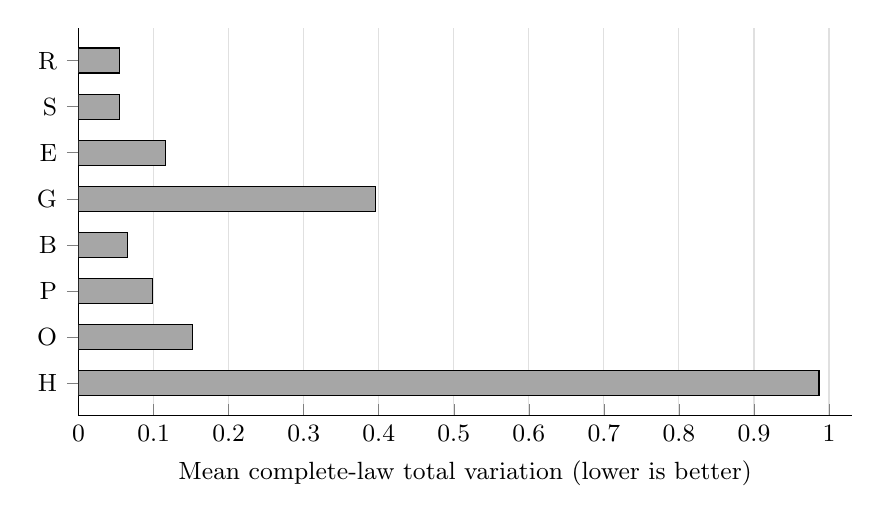
\begin{tikzpicture}
\begin{axis}[width=.94\linewidth,height=6.5cm,xbar,bar width=9pt,
 symbolic y coords={H,O,P,B,G,E,S,R},ytick=data,xmin=0,xmax=1.03,
 xlabel={Mean complete-law total variation (lower is better)},
 axis x line*=bottom,axis y line*=left,xmajorgrids=true,grid style={black!12},
 tick label style={font=\small},label style={font=\small}]
\addplot[fill=black!35,draw=black] coordinates {(0.0549125072011647,R) (0.0549176211694816,S) (0.116209642997078,E) (0.395815864921662,G) (0.0646840524332825,B) (0.0990720629171276,P) (0.15201457568736,O) (0.986651862338821,H)};
\end{axis}
\end{tikzpicture}
\caption{OII-4 observed mean law error on the same 1,152 primary slots. There are no population confidence bars: this is a finite descriptive comparison. R and S nearly coincide.}
\label{fig:means}
\end{figure}

% END figures/mean_tv.tex


B alone passes 1,053 slots, with mean TV 0.064684, 36 all-core fixtures and 11 red failures. The combined portfolio can additionally select ordinary automata on mechanisms where they fit better. H passes only one core slot. This failure is tied to its sparse observed-prefix coverage and uniform sink rule; it is not evidence that retaining history is intrinsically inferior to forgetting it. Nor is the observed ordering universal: the worst-case error still approaches or attains one for the tested methods.

\subsection{What the group-aware branch contributes}\label{p3:c11}
R and S differ only in availability of the two G candidates, with the same calibration objective. They have identical pass, all-core, red-failure and unsafe-merge counts. Their mean TV values are 0.0549125072 and 0.0549176212, respectively, a difference of about $5.1\times10^{-6}$. They select the identical component model on 47 of 48 fixtures. On the remaining joint-encoder fixture, R chooses the group-$0.20$ candidate and S a two-state hidden model. Their respective calibration NLLs are 0.693742 and 0.693802. The largest difference between their core errors there is approximately 0.000304, and no core pass/fail status changes. Thus the identical aggregate pass counts do not conceal offsetting successful and unsuccessful fixtures in this comparison.

The supported conclusion is that the broad gain of the full portfolio is reproduced without the bespoke group-aware branch on this cohort. This is a controlled software ablation using a prespecified secondary portfolio, not a population equivalence or noninferiority theorem. In particular, it does not establish that group-common-law reasoning is useless in other data or merge regimes.

A narrower comparison reinforces this distinction. At the same ordinary compatibility setting $0.05$, the unaugmented automaton passes 541 slots, the group-$0.10$ candidate passes 522, and the group-$0.20$ candidate passes 559. The effects are mixed. Comparing tuned E across four settings with G across two group thresholds would not isolate the group veto. All three fixed-setting candidates remain available in the supplied evidence.

\subsection{Mechanism-dependent gains and regressions}\label{p3:c14}
\Cref{tab:families,fig:families} show the principal tradeoffs. The standard portfolio passes all 48 tests in each of the hidden-belief, mode-register, modular-counter, gated-queue, probe and refractory families. P passes 16, 23, 35, 31, 33 and 24, respectively. These are mechanisms where compact predictive state or a posterior over hidden state is often useful.

The opposite comparison is equally important. On adaptive challenges, R/S pass only 2 of 48 slots while P passes all 48. On delayed receivers they pass 32 versus 48; on finite budgets, 39 versus 48. The predefined streaming features can make particular dependencies easy to express and fit, even when a more general latent architecture contains an exact solution. The results establish contrasting strengths of these implemented procedures, not one representation dominating every other representation.

The family descriptions are post-reveal explanatory labels, not labels supplied to the learner. These small subgroups were not separately powered studies. The full table, including the added checksum, gate and alternating-channel families, is included in \cref{app:results}.


% BEGIN tables/families_main.tex
\begin{table}[tbp]
\centering
\caption{Selected OII-4 mechanism families: large gains and the principal regressions. Each row contains two fixtures and 48 test slots per method.}\label{tab:families}
\small
\setlength{\tabcolsep}{5pt}
\begin{tabular}{lrrrrr}
\toprule
Family & Tests & R & S & B & P \\
\midrule
Hidden belief & 48 & 48 & 48 & 48 & 16 \\
Mode register & 48 & 48 & 48 & 40 & 23 \\
Modular counter & 48 & 48 & 48 & 48 & 35 \\
Gated queue & 48 & 48 & 48 & 43 & 31 \\
Probe-sensitive & 48 & 48 & 48 & 48 & 33 \\
Refractory service & 48 & 48 & 48 & 48 & 24 \\
Adaptive challenge & 48 & 2 & 2 & 2 & 48 \\
Delayed receiver & 48 & 32 & 32 & 32 & 48 \\
Finite budget & 48 & 39 & 39 & 39 & 48 \\
\bottomrule
\end{tabular}
\par\smallskip{\footnotesize These are descriptive subgroups, not separately powered replications. The full family table appears in Appendix~\ref{app:results}.\par}
\end{table}

% END tables/families_main.tex


% BEGIN figures/family_tradeoffs.tex
\begin{figure}[tbp]
\centering
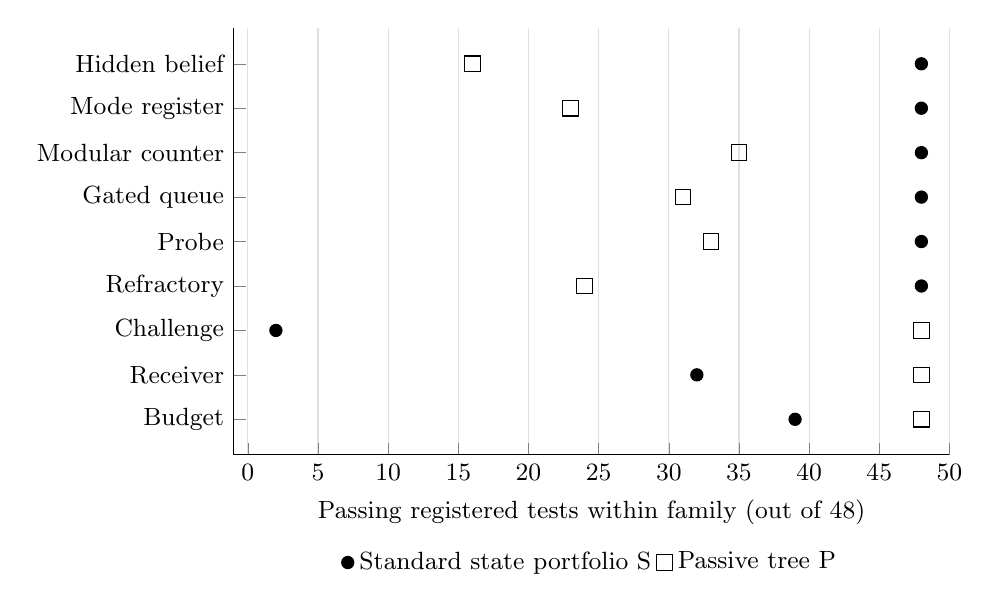
\begin{tikzpicture}
\begin{axis}[width=.88\linewidth,height=7cm,xmin=-1,xmax=50,
 ytick={0,1,2,3,4,5,6,7,8},yticklabels={Hidden belief,Mode register,Modular counter,Gated queue,Probe,Refractory,Challenge,Receiver,Budget},y dir=reverse,
 xlabel={Passing registered tests within family (out of 48)},
 axis x line*=bottom,axis y line*=left,xmajorgrids=true,grid style={black!12},
 tick label style={font=\small},label style={font=\small},
 legend style={at={(.5,-.2)},anchor=north,legend columns=2,draw=none,font=\small}]
\addplot[only marks,mark=*,mark size=2.2pt] coordinates {(48,0) (48,1) (48,2) (48,3) (48,4) (48,5) (2,6) (32,7) (39,8)};\addlegendentry{Standard state portfolio S}
\addplot[only marks,mark=square,mark size=2.8pt] coordinates {(16,0) (23,1) (35,2) (31,3) (33,4) (24,5) (48,6) (48,7) (48,8)};\addlegendentry{Passive tree P}
\end{axis}
\end{tikzpicture}
\caption{The aggregate gain is not uniform dominance. The passive tree control wins on challenges, receivers and finite budgets. All points come from the same OII-4 cohort.}
\label{fig:families}
\end{figure}

% END figures/family_tradeoffs.tex


\subsection{Paired fixture-level descriptions}\label{p3:s01}
Retrospective paired summaries retain the original within-fixture slot weights. For both R/P and S/P, the state portfolio has lower fixture-mean TV on 37 fixtures, P has lower error on ten, and one is tied at tolerance $10^{-12}$. Worst-slot directions are 39, eight and one. All-core outcomes are 19 fixtures on which both pass, 18 state-only, five P-only, and six neither (\cref{tab:paired-fixture}). These counts show how the aggregate advantage is distributed rather than treating 1,152 dependent slots as independent trials.

The median paired fixture-mean difference is only $-0.000595$, whereas the mean R-minus-P difference is $-0.044160$; substantial gains and regressions coexist with small differences on many fixtures. Averaging each of the 22 mechanism-family groups first gives 16 mean-error directions favoring the state portfolio and six favoring P. This second descriptive weighting does not create independent samples. Because the crafted cohort includes related mechanisms and exact twins, no IID sign-test or bootstrap sampling interval is assigned to these counts.

% BEGIN tables/paired_fixture.tex
\begin{table}[tbp]
\centering\caption{Retrospective paired descriptions of the original 48-fixture results. Negative mean differences favor the state portfolio.}\label{tab:paired-fixture}
\small\begin{tabular}{@{}llrrrr@{}}\toprule
Comparison & Metric & State wins & Ties & P wins & Mean difference\\\midrule
R versus P & Fixture mean & 37 & 1 & 10 & -0.044160\\
R versus P & Fixture worst & 39 & 1 & 8 & -0.210943\\
S versus P & Fixture mean & 37 & 1 & 10 & -0.044154\\
S versus P & Fixture worst & 39 & 1 & 8 & -0.210937\\\bottomrule
\end{tabular}
\par\smallskip\footnotesize Tie tolerance is $10^{-12}$. For both comparisons, all-core outcomes are 19 both-pass, 18 state-only, 5 P-only and 6 neither. These crafted, related and twin fixtures do not justify an IID sign-test or sampling-bootstrap interpretation; no inferential $p$ value is reported.
\end{table}

% END tables/paired_fixture.tex


% END sections/04_final_comparison.tex


% BEGIN sections/05_capacity.tex
\section{Capacity, produced candidates and selection}\label{sec:capacity}
\subsection{A post-reveal representational-capacity sanity check}\label{p3:c12}
An unsuccessful fitted model does not reveal by itself whether the architecture lacks capacity. OII-4 permits a direct post-reveal check. Every source generator has at most 16 hidden states and uses the same action/output form as \cref{eq:instrument}. For a target with $n\leq16$, embed its states in the first $n$ coordinates of a 16-state model. Copy every rational joint transition row and each preparation distribution there; set unused states to emit symbol zero and self-loop, with zero initial mass and no incoming mass from the active subspace. The resulting stochastic instrument reproduces every source row on the active subspace and hence every admitted adaptive finite record law.

The saved construction was checked at 3,072 embedded instrument rows and 192 preparation rows. This elementary embedding is an exact capacity sanity check for the \emph{general joint-instrument architecture}, not a novel representation theorem. It is not a theorem about a more restrictive HMM that factorizes emission and transition in a prescribed way. It also does not prove that the specific positive-pseudocount, single-initialization fitting procedure can attain the exact boundary parameters from its finite data.

These exact source-derived parameters were constructed only after reveal and were never included as known-correct training candidates. A strictly positive parameterization can approximate the embedded model by mixing each initial distribution and joint row with a sufficiently small uniform component. The imported coupling bound gives eight-call error at most $1-(1-\eta)^9$ when each such change is at most $\eta$. This is an approximation-capacity statement, not successful identification by the implemented optimizer.

Thus the remaining failures cannot all be explained by insufficient latent-state cardinality. Finite observations, initialization, regularization, local fitting, candidate construction and selection remain possible contributors. Nor does the embedding imply 16 public predictive states: \cref{eq:belief} can attain many distinct posterior values even with a small hidden carrier.

\subsection{Certificates against a produced bank}\label{p3:c07}
Let $\BB_f=\{Q_1,\ldots,Q_J\}$ be the finite bank actually produced on fixture $f$. An episode-level mixture has laws $Q_w^e=\sum_jw_jQ_j^e$, with the same weights across the experiment family. For any legal event $A$ in an experiment $e$,
\begin{equation}
 \TV(P^e,Q_w^e)\ \geq\ P^e(A)-Q_w^e(A)
 \ \geq\ P^e(A)-\max_jQ_j^e(A).
 \label{eq:bank-witness}
\end{equation}
If the final quantity exceeds $\tau$, no mixture in that bank passes this test. This elementary certificate is stronger than observing that one optimizer chose poor weights. It does not exclude an unproduced parameterization in the same mathematical architecture. The witness and probability evaluation are post-reveal diagnostics, not queries available to the opaque learner during selection.


% BEGIN tables/banks.tex
\begin{table}[tbp]
\centering
\caption{OII-4 post-reveal candidate-bank diagnostics. ``Adequate'' in this table means passing all fixed core tests at TV $\leq0.15$.}\label{tab:banks}
\small
\setlength{\tabcolsep}{5pt}
\begin{tabular}{lrrrr}
\toprule
Bank & \shortstack{Passing single\\candidate /48} & \shortstack{Selected\\all-core /48} & \shortstack{Selection\\misses} & \shortstack{Convex-bank\\obstructions /48} \\
\midrule
R & 39 & 37 & 2 & 8 \\
S & 39 & 37 & 2 & 8 \\
E & 28 & 28 & 0 & 19 \\
G & 15 & 15 & 0 & 33 \\
B & 37 & 36 & 1 & 10 \\
P & 25 & 24 & 1 & -- \\
O & 25 & 23 & 2 & 22 \\
\bottomrule
\end{tabular}
\par\smallskip{\footnotesize P selects three trees; O mixes four. The obstruction count 22 refers to the four-tree bank. No P-specific obstruction count is inserted. A missing adequate individual candidate does not exclude an adequate mixture.\par}
\end{table}

% END tables/banks.tex


\subsection{What the counts distinguish}\label{p3:c13}
For both R and S, 39 of 48 fixtures have at least one produced candidate passing every core slot, while the selected predictor does so on 37. The two differences are genuine core-panel selection misses in the post-reveal ranking. They do not establish that the selector could have known the oracle ranking from the available calibration sample. \Cref{tab:selection-misses} identifies both cases. The selected model has lower observed calibration NLL in each; the failure is not a tie-breaking error or evidence that the selector saw the hidden core ranking. The alternative rows are post-reveal comparisons of candidates that had already been fitted.


% BEGIN tables/selection_misses.tex
\begin{table}[tbp]
\centering
\caption{The two R/S core-panel selection misses. Lower calibration NLL wins under the original selector; a core-worst TV at most 0.15 passes.}\label{tab:selection-misses}
\footnotesize
\setlength{\tabcolsep}{5pt}
\begin{tabular}{lllrr}
\toprule
Fixture family & Model & Role & Calibration NLL & Core worst TV \\
\midrule
Leaky occupancy & HMM-8 & Selected & 0.083232 & 0.152781 \\
Leaky occupancy & HMM-16 & Passing alternative & 0.087784 & 0.131943 \\
Coin & IOALERGIA-1.5 & Selected & 0.086455 & 0.196476 \\
Coin & HMM-2 & Passing alternative & 0.086654 & 0.091927 \\
\bottomrule
\end{tabular}
\par\smallskip\begin{minipage}{\linewidth}\footnotesize The rows compare already-produced candidates, ranked after reveal for diagnosis. R and S make the same selections. The coin row shows the lowest-calibration-NLL passing alternative; two additional hidden-state candidates also pass. Full fixture IDs and values are in the audit supplement.\end{minipage}
\end{table}

% END tables/selection_misses.tex


Of the remaining nine fixtures with no adequate individual R/S candidate, eight have a \cref{eq:bank-witness} certificate excluding every convex mixture in the bank. The last case remains unresolved at mixture level: failure of every individual member does not imply failure of every mixture. Consequently, the 11 selected-model failures separate into two selection misses, eight certified produced-bank obstructions, and one case lacking an adequate individual candidate but not excluded by this mixture audit.

The tree bank has 22 such obstructions on the same final cohort, versus eight for R/S. That is a reduction in \emph{produced-bank} insufficiency, not proof that one full architecture is globally more expressive than the other. The capacity construction already shows why those categories must be distinguished.


% BEGIN figures/capacity.tex
\begin{figure}[tbp]
\centering
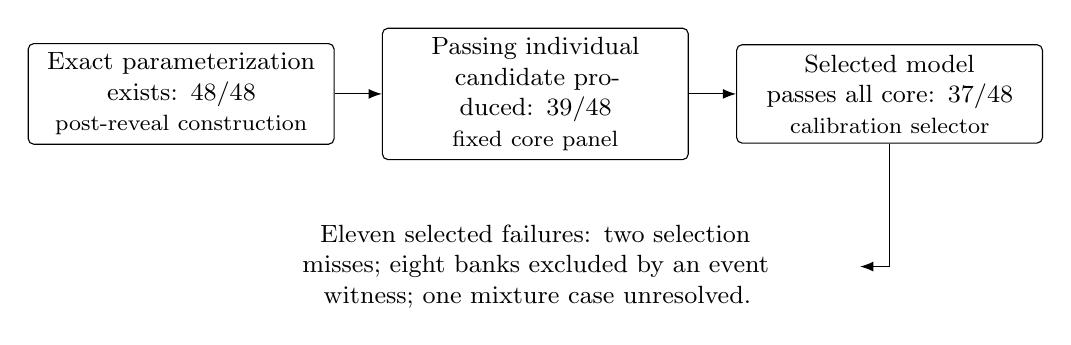
\begin{tikzpicture}[>=Latex,node distance=6mm,box/.style={draw,rounded corners=2pt,align=center,font=\small,minimum height=1.25cm,text width=3.65cm}]
\node[box] (cap) {Exact parameterization\\exists: 48/48\\\footnotesize post-reveal construction};
\node[box,right=of cap] (bank) {Passing individual\\candidate produced: 39/48\\\footnotesize fixed core panel};
\node[box,right=of bank] (sel) {Selected model\\passes all core: 37/48\\\footnotesize calibration selector};
\draw[->] (cap)--(bank);\draw[->] (bank)--(sel);
\node[align=center,font=\small,below=7mm of bank,text width=8cm] (fail) {Eleven selected failures: two selection misses; eight banks excluded by an event witness; one mixture case unresolved.};
\draw[->] (sel.south)|-(fail.east);
\end{tikzpicture}
\caption{Original-budget OII-4 R/S diagnostic separation. The arrows show different questions, not a proof that the learner knew any oracle fact. All counts concern the same 48 fixtures and registered core tests; the separate post-hoc expansion does not overwrite them.}
\label{fig:capacity}
\end{figure}

% END figures/capacity.tex


\subsection{Diagnosis without forced single causes}
There is a hierarchy of questions, not a compulsory single-label taxonomy. An architectural witness answers an existence question. A bank witness excludes a finite collection and its mixtures. A selector miss compares a chosen candidate with other candidates that were produced. None alone identifies the statistical cause of a failed parameter fit.

The frozen study used one start and at most 60 EM updates per size. The post-hoc analysis in \cref{sec:sensitivity} now directly tests a larger budget and finds five selected repairs among its 11 failures. This is evidence of finite-budget sensitivity, not a diagnosis that every residual fit is a local minimum. Insufficient branch evidence, the fixed pseudocount and selection on limited calibration remain possible contributors. Likewise, source models with identical public laws are non-identifiable in their hidden anatomy; that is not the same failure as predicting the public laws incorrectly.

\begin{table}[tbp]
\centering\caption{Failure categories and the evidence needed to distinguish them. Categories may coexist; the table is not a mutually exclusive labeling of all failed fixtures.}\label{tab:failure-taxonomy}
\footnotesize\begin{tabularx}{\linewidth}{@{}>{\raggedright\arraybackslash}p{.22\linewidth}YY@{}}\toprule
Category & What this record establishes & What remains unestablished\\\midrule
Architecture capacity & Exact post-reveal 16-state embeddings for all final targets & Identifiability or convergence of the opaque fitter\\
Produced-bank insufficiency & Eight R/S bank witnesses exclude every produced mixture & Inadequacy of all parameterizations or other candidate generators\\
Parameter estimation & Fitted laws disagree on some source contexts despite architectural capacity & A unique attribution to sampling rather than optimization or regularization\\
Optimization/local fitting & Five selected repairs among 11 targeted failures under the post-hoc expanded budget & Global optimization, a unique causal decomposition, or repair of every remaining miss\\
Model selection & Two R/S candidates were available that passed all core tests but were not selected & That the available calibration observations identify the oracle winner\\
Context/data coverage & Duplicate and calibration-matching specifications; observed panel-to-core failures & A full unseen-policy or all-future generalization guarantee\\
Finite-budget uncertainty & OII-3 confirmation limits and flat confidence objectives & Adequacy from finite nondetection or exact equality from overlapping intervals\\
Operational non-identifiability & Exact public-law twins have different hidden implementations & Permission to excuse wrong predictions of operationally distinct laws\\\bottomrule
\end{tabularx}
\end{table}

% END sections/05_capacity.tex


% BEGIN sections/05b_sensitivity.tex
\section{Post-hoc optimization-budget sensitivity}\label{sec:sensitivity}\label{p3:s02}
\subsection{Why another analysis was warranted}
All 48 original 16-state fits reached the 60-update limit, with one initialization at each size. This records failure to trigger the implemented early-stop rule, not proof of mathematical nonconvergence. It nevertheless leaves a direct finite-budget explanation for part of the produced-bank gap. A subsequent Claude review identified this concern after the original results and audit were known. We therefore froze a separate retrospective protocol and retained the original OII-4 results as the primary study.

The target set is the 11 original R/S all-core failures, including the two selector misses, eight obstructed banks and one mixture-unresolved case. Four originally passing fixtures were chosen by a fixed hash ordering, not by mechanism or error magnitude. This is an outcome-selected diagnostic subset, not a random 15-system replication. No additional interaction data were collected.

\subsection{Fixed fitting and public selection}
For each fixture and each $k\in\{2,4,8,16\}$, six starts were run to at most 600 updates. Start zero repeats the original initialization; five additional seeds are fixed hashes of fixture, size and restart. The instrument family, $0.01$ pseudocounts, fitting and calibration tapes, probability floors and relative stopping tolerance are unchanged. Each run retains the old-cap endpoint as well as its extended endpoint. In total, 360 fits produce 720 saved endpoint records, not 720 independent fits. All 60 original-seed short endpoints reproduce the original parameters exactly.

The principal expanded portfolio $S^+$ contains the original S bank and the 24 extended endpoints for its fixture. Average public calibration NLL selects the model; ties prefer original candidates and then the fixed size/restart order. All 15 batches and selections were committed together before any new core score was computed. The research process had already seen the original failures and source revelations; this local sequencing protects the new selection step, not author-level blindness. The protocol, worker access checks, seeds and commitments are supplied in \cref{app:sensitivity} and the supplement.

Three predeclared auxiliary banks separate aspects of the sensitivity: original S plus the four extended original starts; original S plus the 24 old-cap endpoints from all starts; and the 24 extended HMMs without the old automata. The last comparison changes the bank and is not substituted for $S^+$ when it performs better.


% BEGIN tables/sensitivity_arms.tex
\begin{table}[tbp]
\centering\caption{Post-hoc optimization sensitivity on the 11 outcome-selected failures. Each row uses calibration-only selection; produced counts are evaluated afterward.}\label{tab:sensitivity-arms}
\small\begin{tabular}{@{}lrrrr@{}}\toprule
Procedure & Selected & Produced & Slots & Mean worst\\\midrule
Frozen S & 0/11 & 2/11 & 175/264 & 0.652077\\
Longer, original starts & 3/11 & 5/11 & 201/264 & 0.429132\\
Six starts, old cap & 3/11 & 4/11 & 193/264 & 0.583670\\
$S^+$: six starts, long cap & 5/11 & 7/11 & 212/264 & 0.318750\\
Extended HMMs only & 6/11 & 7/11 & 214/264 & 0.309245\\\bottomrule
\end{tabular}
\par\smallskip\footnotesize All but the last row retain the original eight-candidate S bank. Old and long caps are 60 and 600 updates; the unchanged tolerance can stop a fit earlier. The last row is an auxiliary bank restriction, not the principal sensitivity result. Original 48-system scores are unchanged.
\end{table}

% END tables/sensitivity_arms.tex

\subsection{Five selected repairs; two remaining selection misses}\label{p3:s03}
On the 11 failures, $S^+$ selects an all-core-passing model for five and its expanded bank contains at least one for seven. The frozen S figures on that same subset were zero selected and two produced successes. The selected pass count rises from 175 to 212 of 264 retained slots; mean fixture-worst TV falls from $0.652077$ to $0.318750$. These are post-hoc subset results, not a replacement 48-system headline. The four passing controls all retain their original selected models and all remain passing.

The five selected repairs are checksum protocol, alternating channel, shared budget, delayed receiver and finite budget. Extending only the original starts repairs three; multiple starts at the old cap also repair three, with different membership. The combined expansion repairs five (\cref{tab:sensitivity-arms,tab:sensitivity-fixtures}). The original candidate-production result is therefore materially sensitive to the fitting/search budget. The experiment does not isolate a universal compute effect or certify globally optimal fitting.


% BEGIN tables/sensitivity_fixtures.tex
\begin{table}[tbp]
\centering\caption{Individual outcomes on the 11 original failures. Scores are worst core-slot TV; original labels identify the historical diagnosis, not the cause of fitting failure.}\label{tab:sensitivity-fixtures}
\small\begin{tabular}{@{}llrrll@{}}\toprule
Fixture family & Old type & Frozen S & $S^+$ & Selected & Class\\\midrule
leaky occupancy & Sel. & 0.152781 & 0.246786 & k=08, r=1 & B\\
checksum protocol & Bank & 0.309721 & 0.053293 & k=16, r=2 & A\\
alternating channel & Mix. & 0.506213 & 0.080255 & k=08, r=2 & A\\
shared budget & Bank & 0.467788 & 0.040041 & k=16, r=2 & A\\
receiver & Bank & 0.804479 & 0.016800 & k=08, r=5 & A\\
lock 0 & Bank & 0.999991 & 1.000000 & k=02, r=2 & C\\
budget & Bank & 0.866014 & 0.066692 & k=16, r=5 & A\\
challenge 0 & Bank & 0.939187 & 0.490052 & k=16, r=3 & C\\
challenge 1 & Bank & 0.930191 & 0.315852 & k=16, r=5 & C\\
coin & Sel. & 0.196476 & 0.196476 & old 03 & B\\
lock 1 & Bank & 1.000000 & 1.000000 & old 00 & D\\\bottomrule
\end{tabular}
\par\smallskip\footnotesize A: selected model passes; B: an expanded-bank individual passes but selection fails; C: none passes and best bank worst-error improves by at least 0.01; D: remaining smaller/no improvement. The two locks and challenges are labeled by their original variant. Complete hashed identifiers, fitting iterations and oracle-best candidates are in the supplement.
\end{table}

% END tables/sensitivity_fixtures.tex

The two original selection-miss fixtures remain misses under $S^+$. On leaky occupancy, a new selected eight-state model has core-worst TV $0.246786$, worse than frozen S's $0.152781$, although a produced four-state model reaches $0.065583$. Its public calibration NLL is slightly worse than the selected model's. The old-cap multi-start arm succeeds on this fixture, so additional iterations are not uniformly beneficial after selection. On the coin fixture, the original automaton retains the best observed calibration score and still fails the core panel. The HMM-only auxiliary selector passes it, giving six rather than five repaired fixtures, but discarding old candidates is a distinct bank intervention and not the principal result.

Both locks and both challenges still lack an individually all-core-passing model in the expanded bank. Best worst-slot error improves by at least 0.01 on one lock and both challenges; the second lock changes by less than that descriptive cutoff. The resulting classification is five selected repairs, two selection misses, three improved-but-failing banks, and one smaller/no-improvement bank. The thresholds define reporting categories, not significance or convergence claims.

\subsection{Old certificates and new banks}\label{p3:s04}
The original eight obstruction certificates remain true about their frozen banks. Four of those fixtures now have a passing extended model, showing why the old certificates cannot be carried over automatically. Re-evaluating the original event against every member of each expanded bank gives three rigorous surviving lower bounds: $0.793635$ and $0.999998$ for the two locks, and $0.415180$ for the single-match challenge. Each exceeds 0.15. The same event no longer excludes the offset-match challenge bank, although no individual candidate passes there. Its expanded-mixture adequacy remains unresolved by this nonexhaustive event check.

Of the 360 fits, 219 meet the unchanged stopping tolerance and 141 reach the 600-update cap. Among the targeted failures, 47 of 66 sixteen-state fits still reach the cap. These counts do not support a claim that the enlarged search exhausts optimization. Across all fits, endpoint fitting NLL improves relative to the old-cap snapshot on 286, calibration NLL on 221 and core-worst TV on 182; remaining cases include ties and deteriorations. The different counts, and the explicit selector misses, rule out treating likelihood improvement as guaranteed downstream adequacy.

\subsection{What fails in the adaptive challenge}\label{p3:s05}
The revealed challenge generator alternates a random challenge and an immediate response. At phase zero it emits $j\in\{0,1,2,3\}$ uniformly and retains $(j,b)$, where $b$ is a prepared bit. At the next call it emits $(2+b)\mathbf1\{a=(j+d)\bmod4\}$ and returns to the challenge phase; $d\in\{0,1\}$ is the variant. Public actions and outputs use the saved permutations and XOR encoding. Thus the challenge value requires one-call retention, while the prepared bit persists through the episode. This is not a long-delay challenge mechanism.

Both selected tree controls use exactly the preparation code, time modulo two and previous output as split features, together with action-conditioned rows. Those features expose the relevant distinctions directly. Each original fitting tape contains 3,840 response events, covers all 64 preparation/challenge/action rows, and has at least 39 or 45 observations per row, respectively. The observed failure is not absence of every instance of a required response combination.

The frozen selected models both have eight latent states. After the first challenge, their posterior vectors for different challenge values at a fixed preparation have TV distances above 0.997. They therefore do not simply collapse or forget the observed challenge. Their predictions instead mix the two prepared-bit-dependent matching responses: the correct matching-response probability averages $0.5037$ and $0.4988$, versus above $0.9997$ for the tree controls (\cref{tab:challenge-diagnostic}). Direct bit-contrasted traces are given in \cref{tab:challenge-traces}.


% BEGIN tables/challenge_diagnostic.tex
\begin{table}[tbp]
\centering\caption{Source-revealed challenge diagnosis after selection. The first-response probabilities average equally over four preparations and four challenges, choosing the matching next action.}\label{tab:challenge-diagnostic}
\small\begin{tabular}{@{}lrrrr@{}}\toprule
Fixture & Frozen S & Tree P & $S^+$ & $S^+$ core worst\\\midrule
Challenge 0 & 0.5037 & 0.9998 & 0.8667 & 0.490052\\
Challenge 1 & 0.4988 & 0.9998 & 0.9895 & 0.315852\\\bottomrule
\end{tabular}
\par\smallskip\footnotesize The first three numeric columns are probability assigned to the deterministic correct matching response; the source value is one. They are diagnostic conditional probabilities, not extra primary tests. Both new selected models have 16 latent states; the original selected models have eight.
\end{table}

% END tables/challenge_diagnostic.tex

The selected sixteen-state extensions improve those matching-response averages to $0.8667$ and $0.9895$. Nevertheless, core-worst errors remain $0.490052$ and $0.315852$, and their selected core-pass counts are one and zero. On original-core prefixes, response-row TV decreases, while the error in the nominally uniform challenge-output rows increases. This localizes observed prediction defects more precisely than ``insufficient memory,'' without proving a unique statistical cause. The receiver preserves a prepared bit behind a native delay and the budget fixture carries a remaining-token count; both selected failures disappear under the same optimization expansion. Their common repair does not establish that they shared the challenge's response-mixing mechanism.

% END sections/05b_sensitivity.tex


% BEGIN sections/06_development.tex
\section{Why the earlier repair stages did not close discovery}\label{sec:development}
The preceding final comparison was motivated by a sequence of failures, not by an a priori claim that one bespoke learner should win. This section explains those decisions while preserving each study's own denominator. Full tables and allocation details appear in \cref{app:results,app:chronology}.

\subsection{Known-model implementation conformance}\label{p3:c02}
RRI implemented owned registers, queues, deadlines, local/shared randomness, consumable counters and retained monitoring records in an event runtime. A separate oracle, not importing that runtime, specified the nominated exact laws. The study executed 1,557,504 fixed-seed trials over 225 conditions, with 70 derived metrics, 27 exact check groups and five supplementary checks of already registered obligations. All 225 row-law and 70 metric intervals covered the exact values in that run. This is one coverage event under the recorded pseudorandom realization, not an estimate of a nominal coverage rate.

The tests include failure of early decoding from late records, adaptive amplification of a fixed-input discrepancy, distinct SWAP simulation budgets under different communication/randomness resources, and preservation of one-use resource state. They provide known-model software conformance to the imported contract. They are neither blind identification nor independent physical confirmation. RRI's trials are not interchangeable with the public-call counts used in OII.

\subsection{Shallow history inference: OII-1}\label{p3:c03}
OII-1 uses 28 opaque fixtures and a 420-slot common core. Active and passive acquisition each receive 9,216 calls and 4,736 reset episodes per fixture. Both first collect balanced one-step observations, then longer discovery and calibration-validation episodes. The selected model retains suffix depth zero through three, with optional preparation and clock. Joint-output count smoothing and a complexity-penalized NLL selector define a bounded engineering procedure.

The selected active predictor passes 281 of 420 core slots and all slots on 12 fixtures; the selected passive predictor passes 266 slots and all slots on 13 fixtures. Their mean TV upper values are 0.223891 and 0.218708. Thus active acquisition improves pass count but not every metric. Selected-model red failures occur on 15 and 13 fixtures, respectively. Matched memoryless and factorized-output controls are weaker in the reported core aggregates (\cref{tab:oii1}).

OII-1 also has a 705-slot expanded panel containing learner-selected probes. It must not replace the common-core denominator. Its initial merge audit sampled different histories for the two learners: 56 versus 131 separating witnesses arose among 79 versus 168 unequal-belief pairs. These are not directly comparable false-merge rates on a common population. Later studies introduced common witness panels. A post-score auxiliary horizon/clock correction is preserved, with the primary scores unchanged.

\subsection{Representation-rich repair: OII-2}\label{p3:c04}\label{p3:c05}
OII-2 changes the learner to 100 public streaming features and conditional joint-output trees, with explicit registers implementing each retained feature. The active procedure proposes histories it currently merges, attempts legal prefix replay, tests a fixed suffix event on fresh samples, and protects a distinguishing feature after a sufficiently large confirmed separation. Failed replay attempts consume budget; there is no reset to a privileged hidden state.

On its 36-fixture, 720-slot common panel, the rich active procedure passes 633 slots, versus 442 for the old active learner, with mean TV upper decreasing from 0.263312 to 0.086537. Both representation and observation allocation changed, so this supports the combined richer procedure, not an isolated causal effect of the dictionary. The rich passive method has fewer passing slots (630) but lower mean error (0.078505) and fewer red failures (11 versus 14).

The especially informative ablation refits on the \emph{same active data} without the explicit confirmed-counterexample constraints. It passes 639 slots with mean TV upper 0.080784, slightly better than the constrained fit. This does not remove the observations acquired during counterexample search and therefore cannot identify the value of those queries separately. The conclusion is no demonstrated extra benefit from these explicit fitting constraints on the realized dataset, not a theorem that counterexample guidance has no value.

The search conducted 46 conditional tests and confirmed six refutations across three fixtures. It spent 4,719 replay attempts to obtain 2,290 accepted continuation samples. The confirmed distinctions survived source audit and remained represented. The mechanism was therefore not simply producing false witnesses. Rather, a true witness does not determine which global repair is best. A post-score four-history example shows that a valid separating refinement can improve likelihood yet increase worst-context TV from $1/2$ to $2/3$ (\cref{app:likelihood}). That is a counterexample to an implication, not a unique causal diagnosis of the empirical misses.

\subsection{Objective alignment and finite-bank limits: OII-3}\label{p3:c06}
OII-3 tests likelihood, empirical minimax, uncertainty-aware and safe selectors over finite candidate banks. The scored V2 cohort has 42 fixtures and 1,008 core slots. Three new acquisition lanes use counterexample replay, disagreement exploration without replay, or passive actions. They share a base grammar and total call allowance but obtain different observations. Two inherited OII-2 controls spend the same total allowance according to their original allocation. The new lanes reserve 3,840 of 9,216 calls for a dedicated risk-calibration panel; they do not give the same fitting data as the controls.

Within the counterexample lane, the likelihood mixture passes 836 slots with mean TV upper 0.109167. The same eligible-bank empirical minimax mixture passes 806 with mean 0.121151. Its mean fixture-worst error is slightly lower, 0.368416 versus 0.373416, so the comparison is mixed rather than a failure on every objective. The confidence-upper-bound selector passes 714. The older passive control remains strongest on the headline pass and mean-error measures in the selected comparison, but that is a total-budget procedure comparison, not objective-only evidence.

Post-reveal event witnesses exclude every mixture in the supplied banks on 20 counterexample-lane fixtures, 22 disagreement-lane fixtures and 20 passive-lane fixtures. For those banks, no selector can choose an adequate mixture for every core test. This is a restriction on the produced candidates, not a general impossibility for minimax learning or the full underlying model grammar.

\subsection{Measured-panel safety does not transfer automatically}\label{p3:c08}
The safe selector uses simultaneous risk bounds on one measured panel. If for all candidate laws $L(Q)\leq R_{\E_0}(Q)\leq U(Q)$ on the confidence event, replacement under
\begin{equation}
 U(Q_{\mathrm{new}})+\eta\leq L(Q_{\mathrm{old}}),\qquad \eta=0.001,
 \label{eq:safe}
\end{equation}
guarantees $R_{\E_0}(Q_{\mathrm{new}})+\eta\leq R_{\E_0}(Q_{\mathrm{old}})$ on that same panel. Comparing upper bounds alone would not suffice. The short conditional argument is recorded in \cref{app:safe}.

Four distinct lane/fixture replacements were accepted. All improved their measured-panel maximum, but all worsened core mean error and one worsened core maximum error. \Cref{tab:safe} shows that latter case. There is no contradiction with \cref{eq:safe}: it does not certify unmeasured contexts. The example separates validity of a panel certificate from coverage of the interaction space needed for later use.


% BEGIN tables/safe_example.tex
\begin{table}[tbp]
\centering
\caption{OII-3 CE-lane safe replacement on fixture \texttt{v\_75b71402029f9b}. The certificate concerns its measured panel.}\label{tab:safe}
\small
\setlength{\tabcolsep}{5pt}
\begin{tabular}{lrr}
\toprule
Quantity & Incumbent & Replacement \\
\midrule
Panel maximum TV & 0.923033 & 0.618318 \\
Core mean TV upper & 0.268199 & 0.332146 \\
Core maximum TV upper & 0.889983 & 0.921409 \\
Core passes /24 & 14 & 10 \\
\bottomrule
\end{tabular}
\end{table}

% END tables/safe_example.tex


\subsection{Counterexample completeness and confidence resolution}\label{p3:c09}
OII-3 also exposes two limitations of this particular refinement design. First, pairwise separation above $2\tau$ is a sufficient merge refutation but not a complete class-adequacy test. Three laws can all be within pairwise distance 0.24 while no common predictor is within 0.15 of every law; their optimal common radius is 0.16 (\cref{app:group}). This motivates, but does not empirically validate, OII-4's group-aware heuristic.

Second, a valid confidence objective can fail to distinguish available models. Of 126 new-lane panels, 28 optimized upper bounds are at least 0.9 and none is at most 0.15. Exact post-score certificates show the chosen upper-bound objective is constant over the whole convex bank on 74 panels. This concerns one conservative construction and budget, not all uncertainty-aware learning.

The V2 counterexample lane conducted 29 tests, confirming one and leaving 28 unresolved, with 3,357 attempts and 1,873 accepted samples. A single confirmed fixture provides little evidence for a general incremental advantage. Taken together, OII-1--3 identify useful failure modes but do not establish that better counterexamples or a more appropriate objective alone solve finite opaque identification.

% END sections/06_development.tex


% BEGIN sections/07_adversarial.tex
\section{Adversarial contexts, composition and uncertainty}\label{sec:adversarial}
\subsection{Legal postcommit witnesses}\label{p3:c15}
OII-4's scorer evaluates 32 candidate contexts per fixture after commitment, retaining the strongest found event for each method/fixture. The context grammar is fixed, while the event selection is privileged by knowledge of the source and candidate laws. Every challenge uses the original public preparation/action/output contract and at most eight calls. The 1,536 candidate slots contain 1,534 distinct literal specifications; 51 slots match a core specification and 49 match calibration. Comparing complete finite policy behavior instead gives 1,532 distinct behaviors, 55 core-matching slots and 51 calibration-matching slots. Every method receives the same 32-context search pool on each fixture. Red results therefore are not a wholly disjoint second holdout.

There are 384 selected event records, one for each of eight methods on 48 fixtures. The original audit recomputed those events using exact integer outward rounding of the canonical saved-parameter laws. Its maximum interval width is $6.117\times10^{-11}$, and the certified above-0.15 failures agree with the reported counts. The present hostile audit additionally recomputed all 384 selected events with a separately written evaluator and integer-outward calculation; the largest new event interval width, including the bank-event checks, is $6.246\times10^{-13}$. It also reevaluated the full original 1,536-context red pool and recovered every saved method-specific maximum within $7.8\times10^{-16}$. The historical certificate width above and the new audit width refer to different arithmetic runs, not new experimental observations. A finite strongest-found event is not an exhaustive maximizer over all policies or a certificate of the shortest distinguishing horizon.

For the common merge audit, equal-clock three-call prefixes from two preparations and four constant-action policies are compared under one-call continuations. A fixed path cap limits the witness panel, not the primary score calculation. The source audit identifies 8,478 pairs with true continuation gap above 0.30. R and S collapse 28 of these pairs, E 820, G 2,872, P 153, O 110 and H 3,682. B has zero identical retained-state-key violations on this panel, despite nonzero predictive error. A continuous posterior key can avoid exact equality without being correct or minimal.

For any two true continuation laws $P,P'$ and common prediction $Q$, the triangle inequality gives
\begin{equation}
 \max\{\TV(P,Q),\TV(P',Q)\}\geq\tfrac12\TV(P,P').
 \label{eq:merge-witness}
\end{equation}
That justifies each sufficient pair refutation. It does not justify treating every unrefuted merge as safe or different sampled panels as one population rate.

\subsection{Supplementary composition}\label{p3:c16}
Eight pairs were specified during OII-4 fitting, before hidden scoring, by pairing the first 16 lexicographically sorted opaque IDs. They are disjoint module carriers, not overlapping physical resources. A causal controller makes eight alternating global calls, four to each module, with actions determined by pair index, tick and the last global output. The composition data are separate from the 1,152 core slots.

R and S pass all eight supplementary composition tests. Seven pairs have both local modules passing their entire core panels, and all seven also pass the composed test. B passes all eight, while E, P and O pass six, three and one, respectively (\cref{tab:composition}). The composition pairs were neither chosen after finding local successes nor a representative sample of all legal wirings.

These are finite supplementary observations, not a learned uniform \RRC{} certificate. A local finite panel may omit a conditional distinction used by a different controller. Conversely, a model failing a long local test can pass a shorter particular composition. Neither outcome changes the hypothesis requirements of the imported substitution theorem.


% BEGIN tables/composition.tex
\begin{table}[tbp]
\centering
\caption{OII-4 supplementary composition: eight separately specified pairs.}\label{tab:composition}
\small
\setlength{\tabcolsep}{5pt}
\begin{tabular}{lrrr}
\toprule
Method & Passes /8 & Both modules all-core & Those pairs passing \\
\midrule
R & 8 & 7 & 7 \\
S & 8 & 7 & 7 \\
E & 6 & 2 & 2 \\
G & 0 & 0 & 0 \\
B & 8 & 5 & 5 \\
P & 3 & 0 & 0 \\
O & 1 & 0 & 0 \\
H & 4 & 0 & 0 \\
\bottomrule
\end{tabular}
\end{table}

% END tables/composition.tex


\subsection{Exact public-law twins}\label{p3:c17}
Distinct source carriers can produce identical complete laws through the admitted interface. OII-4 includes four such pairs, with exact post-reveal row/preparation mappings checked in the preserved audit. They are deliberate dependent controls, not eight unrelated statistical replicates. Equal public behavior does not identify a unique microscopic representation, and splitting a pair by a private implementation name would not be an identification success.

The exact equality result is supplied by source-level proof after reveal. The learner's finite nondetection is not that proof. The same distinction governs the earlier stages' equivalent-carrier controls: an opaque procedure may reasonably leave implementation identity unresolved even when it predicts the public behavior well. Public-law equivalence is therefore a boundary on what is to be learned, not an excuse for failures on laws that are genuinely different.

% END sections/07_adversarial.tex


% BEGIN sections/08_related_reproducibility.tex
\section{Related work, reproducibility and external validity}\label{sec:related}
\subsection{Methodological antecedents}
Reactive probabilistic learning and model checking already motivate inducing finite state models from alternating inputs and outputs \cite{Mao2012MDP}. Learned networks of communicating I/O automata provide a related relational setting \cite{MaoJaeger2012}. The local IOALERGIA adaptation executed here follows a subset of this methodological lineage, with publicly documented AALpy source as its implementation reference \cite{AALpySource}. Upstream implementation equivalence was not proved, and the historical source reading was not pinned to an immutable upstream commit. The adaptation's precise reset typing, smoothing and unknown-sink rules therefore form part of the tested algorithm.

Observation-table active MDP learning has both ideal and sampled-access treatments \cite{Tappler2019}. Probabilistic black-box checking also combines learning, candidate-counterexample synthesis and statistical validation \cite{Shijubo2023}. Those works are close antecedents for the general repair loop, not methods executed in this benchmark. No superiority over either is inferred. The OII-2/3 contribution is the recorded costed witnesses, matched fitting controls, and the limits they expose in these particular implementations.

Hidden-state likelihood estimation has a long-standing basis \cite{Baum1970}, and input--output predictive structures have their own theory \cite{Barnett2015}. Predictive-state representations (PSRs) make a different representational choice: state is expressed through action-conditional predictions of observable future tests \cite{Littman2001PSR}. The system-dynamics-matrix account clarifies the relation between predictive, finite-history and hidden-state representations \cite{Singh2004PSR}. Spectral transformed-PSR learning provides a route from action--observation data to prediction and planning under its specified assumptions \cite{Boots2009PSR}. Our controlled joint-instrument learner retains a posterior over fitted latent states; it is not an implemented PSR learner. Neither that spectral PSR method nor spectral HMM identification \cite{Hsu2012} was executed as a comparator. Context/credit diffusion in Markovian models \cite{Bengio1995} is relevant background, while the source-backed challenge diagnosis in \cref{p3:s05} establishes the narrower observed response-mixing defect.

Finite-data overfitting of a model-selection criterion and subsequent evaluation bias are also established issues \cite{Cawley2010}. Adaptive-data-analysis work studies controlled holdout reuse under explicit assumptions \cite{Dwork2015}. We implement neither a protected-reuse mechanism nor their generalization bounds. The present distinction between calibration specifications, sampled observations and withheld law scores is instead a concrete provenance audit of this record. It neither labels all adaptive development as leakage nor treats withholding scores as complete protection from shared-design bias.

Finally, intervention-respecting causal abstraction, coarse-graining of open Markov processes and quantitative probabilistic composition already have independent mathematical foundations \cite{Rubenstein2017,Baez2018,Gebler2013}. Directed statistical deficiency has also been used for feature quality \cite{vanRooyen2014}. The companion paper \cite{RodgersPaper2} supplies the particular marked-instrument contract used here. We do not claim to originate those general frameworks or to re-prove their theory in this empirical manuscript. The companion intervention-law study \cite{RodgersPaper4} examines conditional identification of binary realizations, recoding obstructions and a bounded SPC-2/IIT comparison. Its identification results are distinct from the finite-budget learning and selection outcomes reported here; it was not an executed benchmark comparator.

\subsection{Source-to-manuscript reproducibility}\label{p3:c22}
The present manuscript supplement preserves the pre-audit manuscript ZIP and the authoritative evidence-freeze ZIP unchanged, along with the canonical score exports, table-generation code, source hashes, and the updated claim-to-section map. The freeze itself contains the selected historical protocols, public data, committed models, source-reveal diagnostics and verification reports. The supplied companion-theory source is retained by hash. The companion publications are identified by the DOIs recorded in the bibliography; those identifiers do not replace the hashes of the supplied source snapshots.

The verification stages have distinct scopes. Original-stage checks evaluated record laws and finite controls. The evidence freeze reaggregated saved scores and checked selected structural and chronology claims; drafting regenerated tables and compiled the paper. The subsequent hostile audit separately reconstructed all OII-4 core laws from preserved generators and fitted parameters. This revision adds genuinely new, retrospective fits on old data, checks their short endpoints against the original code, and re-evaluates their core predictions with a separately written batched forward routine. None of these stages is an independently authored benchmark.

The original OII-1--3 mean values include conservative scoring allowances; the OII-4 scorer enumerates the rational source support without path truncation and evaluates learned laws numerically. Its selected event certificates are a separate outward-rounded check. Exact arithmetic on exported decimal scores verifies aggregation; it does not retrospectively make every process-law calculation an exact rational optimization. Similarly, byte-identical model reproduction after removing timing fields does not prove algorithmic generalization.

A bounded methods check during drafting found early stopping in the already frozen EM routine. The original code uses one initialization per latent size and at most 60 iterations, stopping after at least 12 when successive recorded training NLL values satisfy the prescribed relative tolerance. All historical model probabilities, selectors and scores are untouched. The amendment, the 192 metadata records and the original code hashes are distributed with the manuscript.

\subsection{Complexity and cost}
The final suite has 720 fitted component models, shared by overlapping portfolios. Same acquisition data does not mean identical computation. The ordinary automata have median exported size seven including reset type and sink; the unmerged history control has median 4,676.5. The B selector's median latent dimension is six, but its live state is a belief vector plus clock. P has median four retained streaming registers. These are different units and are reported by model type rather than combined into a single complexity ranking.

Recorded component-fitting durations also overlap across portfolios. The median sum of E+B fitting durations is 1.561810 seconds per fixture; adding G gives 5.109376 seconds. These are original execution records, not newly timed end-to-end pipelines, hardware-independent complexity bounds or a compute-matched comparison. Selector and orchestration overhead is not uniformly included. Full size and timing conventions appear in \cref{app:cost}. The separate sensitivity used 360 fits and 119,521 EM updates; the sum of recorded worker durations was 1,248.15 seconds with four concurrent single-threaded workers. This is recorded fitting/endpoint-evaluation time, not a compute-matched comparison against the original full suite.

\subsection{Limits on causal and external claims}
The results apply to a finite synthetic cohort, fixed horizons, fixed preparation/action alphabet and the recorded observation budgets. Longer dependencies, richer ports, different reset access, nonstationarity, arbitrary nondeterministic schedulers and natural-system noise were not covered. The sensitivity varies starts and iteration budgets on an outcome-selected subset but still uses one data realization per fixture, so it does not estimate variability over repeated training tapes. Related fixtures and exact twins intentionally violate any naive independent-slot interpretation.

No study establishes that active acquisition, explicit counterexample constraints or minimax fitting is uniformly better. The R/S result is a secondary matched ablation of a specific candidate addition, not evidence that every possible group criterion has zero value. Capacity, fitting and selector diagnoses remain restricted to the specified candidate families and registered panels. Missing witnesses leave uncertainty; the finite core and composition tests do not establish all-context adequacy.

The same-author generator and learner design is the largest external-validity limitation. Restricted programs and local locks reduce direct hidden-data access along the inspected path, but do not remove conceptual leakage, inherited design preferences or shared implementation errors. Independent code/mathematical scrutiny and an independently authored opaque benchmark would strengthen the result. The latter is a separate versioned study: benchmark authors should work from the public contract without tuning to the frozen learner's scored failures, and a separate scorer should control reveal. The present retrospective additions do not alter that requirement.



The post-hoc protocol was set after the old outcomes and critique were known. Targeting failures, reusing calibration and reporting only four hash-selected passing controls prevents a whole-cohort success or safety estimate for $S^+$. More candidates also create more opportunities to fit calibration noise. Sixty-seven of 90 extended sixteen-state runs hit the new cap, and no global optimum or absence of additional budget effects is established. These qualifications belong to the sensitivity interpretation, not to a retroactive change of the original primary scores. No study here supplies consciousness evidence; the companion's phenomenal claims remain separate.
\paragraph{Funding and collaboration.}
This research was conducted independently by Jeremy Rodgers without external research funding. The author welcomes collaboration on independent mathematical review, computational replication, physical implementation and empirical testing, particularly where specialist expertise, equipment or institutional resources are required.

\paragraph{AI assistance and author responsibility.}
OpenAI GPT-family models, including configurations referred to in the research record as Astra, assisted with mathematical exploration, experimental software, analysis, literature work and manuscript drafting/editing under the author's direction. Anthropic Claude and Google Gemini contributed critique and publication-planning discussion in the surrounding programme. The actual scored learners were the software algorithms described here, not those language models acting as independent investigators. The author retains responsibility for claims, sources and the released manuscript. AI-assisted checking is not represented as independent human review, proof-assistant verification or investigator replication.

% END sections/08_related_reproducibility.tex


% BEGIN sections/09_conclusion.tex
\section{Conclusion}\label{sec:conclusion}
The original same-evidence comparison shows a useful finite advantage of standard probabilistic automata and controlled hidden-state models over the tested tree controls. A prespecified secondary portfolio without the bespoke group-aware candidates reproduces the full portfolio's broad performance. The paired fixture directions support that aggregate description while preserving severe mechanism-specific reversals.

The capacity check is elementary but diagnostically useful: the chosen general architecture can express every target. Under the original budget, produced individual successes cover 39 of 48 fixtures and calibration selection succeeds on 37. These figures are properties of the executed search, not a structural discovery impossibility. The separate post-hoc six-start, 600-update analysis repairs five of the 11 selected failures and produces passing candidates on seven. Two public-selection misses persist, including one deterioration, while both locks and both challenges still lack an individually passing expanded candidate. Three old events also certify obstruction of their expanded banks.

The challenge diagnosis refines the failure mechanism. The selected old models distinguish observed challenges, but mix responses that depend on the prepared bit; the tree exposes preparation, phase and last output directly. Increased fitting effort improves that discrimination without yet making the full challenge laws adequate. Thus capacity, finite-budget search, selection and record-law validation remain distinct, with an important part of the original gap now demonstrably budget-sensitive.

The original panels, context duplicates, calibration overlaps, secondary designations and pre-score repairs remain part of the reported evidence. The retrospective additions neither replace those results nor constitute new external confirmation. The next validation steps are methods review and independently authored benchmarks, not another rebranding of this same-author finite study as a universal interface-learning result.

% END sections/09_conclusion.tex

\FloatBarrier
\appendix

% BEGIN sections/appendix_a_methods.tex
\section{Implementation details and the exact role of each learner}\label{app:methods}
This appendix specifies the implemented OII-4 methods, rather than transferring guarantees from a similarly named published algorithm. The evidence package retains the full original code, settings, committed model bundles and fitting logs. The principal routines are \texttt{state\_learning.py} and \texttt{study\_learner.py}; a fresh implementation should reproduce those choices before interpreting a discrepancy as replication failure.

\subsection{Public evidence and calibration selection}
Each fitting episode begins at one of four public preparations and contains eight action/output pairs. The 960 fitting episodes cycle through the preparations; their four-valued actions are sampled uniformly. The 24 calibration policy specifications comprise four constant policies, eight fixed action words, eight reactive policies and four history-dependent policies, with eight independent reset episodes per specification. In the saved policy grammar the latter are named \texttt{history\_xor}, but their implemented action at zero-based tick $t$ is $(\text{offset}+\sum_{j<t}o_j+t)\bmod4$, a modular sum of output symbols rather than bitwise XOR. This names the existing implementation accurately without changing any policy or observation. These 192 episodes are separate from the fitting episodes, but their policy descriptions need not be absent from the later oracle panel.

For a candidate $M$, selection uses the average conditional next-output negative log likelihood
\begin{equation}\label{eq:nll}
 \ell_{\rm cal}(M)=-\frac{1}{N_{\rm calls}}
 \sum_{e\in\mathcal D_{\rm cal}}\sum_{t=0}^{7}
 \log\!\left(\max\{p_M(o_t\mid h_t,u_t),10^{-300}\}\right).
\end{equation}
The action is conditioned on; the candidate is not rewarded for predicting the externally chosen policy. Equal validation values are broken by original candidate index. R selects from indices 0--9; E from 0--3; G from 4--5; B from 6--9; S from 0--3 and 6--9; P from 10--12; H uses index 14. O separately mixes indices 10--13. Candidate fitting uses only the training tape. The public calibration tape selects the exported candidate or mixture; hidden-law scoring follows commitment.

\subsection{The local IOALERGIA adaptation}
The input/output frequency prefix tree begins with a synthetic reset symbol $4+p$ and acknowledgement zero for preparation index $p\in\{0,1,2,3\}$. The root remains a distinct reset-only operating type. It is not merged with live nodes. Subsequent edges carry the full pair $(u,o)$, with $o\in\{0,1,2,3\}$ encoding both output bits jointly.

The red/blue procedure considers the shortest blue prefix, with lexicographic tie breaking, and compares it with red nodes in the same order. Original prefix counts remain available for recursive compatibility tests after folding. For two nodes with positive counts $n_1,n_2$ for an action, each output frequency difference is compared with
\begin{equation}\label{eq:compatibility}
 \left(n_1^{-1/2}+n_2^{-1/2}\right)
 \sqrt{\tfrac12\log(2/\varepsilon)}.
\end{equation}
Compatibility is also required on common original child edges. Missing or unobserved actions do not establish a distinguishing law. Accepted nodes are folded, their observed counts combined and compatible successor structure identified. The four E variants use $\varepsilon\in\{0.01,0.05,0.5,1.5\}$. These settings are tuning parameters of the published-style compatibility test, not a simultaneous confidence level for all adaptively selected merges.

The exported automaton has deterministic successor labels conditional on $(u,o)$ and stochastic output rows. A count vector $(c_0,\ldots,c_3)$ is smoothed as
\begin{equation}
 \widehat p(o\mid s,u)=\frac{c_o+1/256}{\sum_jc_j+4/256}.
\end{equation}
An unobserved successor goes to an explicit sink with uniform output rows and self-loops. The H control exports the unmerged tree with the same smoothing and completion rule. Its poor scored performance is evidence about sparse-prefix prediction with this fallback, not a theorem that storing complete history is intrinsically inferior.

This is a local stochastic-Mealy-machine adaptation of the IOALERGIA family, informed by its published formulation and AALpy source \cite{Mao2012MDP,MaoJaeger2012,AALpySource}. The audit compared the recursive common-child test, Hoeffding expression, red/blue ordering and folding with the available upstream source. Reset-only typing, count smoothing and the uniform unknown sink remain local choices. The upstream branch cited is mutable; the local executed source is frozen by hash, but the record does not identify an immutable historical upstream commit. No end-to-end equivalence with the upstream package or transfer of its asymptotic guarantees is asserted.

\subsection{The group-aware variants}\label{app:group}
G augments the $\varepsilon=0.05$ pair test with a proposed merged-group test. For each live action, original member prefixes with at least 12 samples supply empirical four-outcome laws $\widehat p_i$ and tuning allowances $a_i=0.35/\sqrt{n_i}$. The procedure bounds or solves
\begin{equation}\label{eq:groupfit}
 \min_{q\in\mathcal S_4}\max\{0,\max_i[\TV(\widehat p_i,q)-a_i]\},
\end{equation}
where $\mathcal S_4$ is the four-outcome probability simplex. A pair lower bound can reject early; for two members the corresponding radius is explicit. For larger groups, all nonempty proper output subsets give the finite linear-program representation of TV. A candidate merge is rejected if the value exceeds the selected threshold, $0.10$ or $0.20$, up to the implemented $10^{-10}$ numerical comparison tolerance. Common folded successors are also checked. The code labels rejections as heuristic, not confidence-certified.

Sparse prefixes can therefore escape the group test. In addition, a changed merge order can change later proposals, so G need not be a simple finer partition of the E model. These are implementation facts relevant to the poor group-only result and mixed fixed-compatibility comparison. The allowances in \cref{eq:groupfit} are not licensed as familywise confidence bounds.

There is nonetheless a valid reason not to equate pairwise nondetection with group adequacy. For $m$ laws
\begin{equation}
 P_i=(1-s)\delta_0+s\delta_i,\qquad i=1,\ldots,m,
\end{equation}
all pairwise TV distances are $s$, while
\begin{equation}\label{eq:group-radius}
 \inf_Q\max_i\TV(P_i,Q)=s(1-1/m).
\end{equation}
The symmetric center with mass $1-s$ at zero and $s/m$ at each private atom attains this value. To prove the lower bound, average any center over permutations of the private atoms, which cannot increase the convex maximum risk. If its total private mass is $v$, the overlap with a target is at most
$\min\{1-s,1-v\}+\min\{s,v/m\}$, maximized at $v=s$, giving the claimed radius. Mass outside the displayed atoms cannot increase overlap. Thus $s=0.24$, $m=3$ gives radius $0.16$ even though every pair distance is below $2(0.15)$. The exact counterexample does not certify the sampled merge heuristic.

\subsection{Controlled hidden-state fitting and stopping}\label{app:em}
For each $k\in\{2,4,8,16\}$ the method fits four preparation distributions $\pi_p$ and the general joint instrument $K_{u,o}(s,s')$. It does not impose the factorization $T_u(s,s')E(o\mid s')$. This distinction is necessary for the capacity construction in \cref{sec:capacity}.

One initialization is used per size. Its seed is the first four bytes of the SHA-256 digest of the fixture identifier concatenated with \texttt{:HMM:} and the size. Each action/current-state joint row is initialized by a Dirichlet distribution with concentration $0.7$ per $(o,s')$ coordinate; each prepared law uses concentration one per coordinate. Standard scaled forward/backward calculations condition on the observed action sequence. If $f_t$ is the normalized forward row and $c_t=f_tK_{u_t,o_t}\one$, the expected transition count is proportional to
\begin{equation}
 \xi_t(s,s')=
 \frac{f_t(s)K_{u_t,o_t}(s,s')b_{t+1}(s')}{c_t},
\end{equation}
where $b_t$ is the correspondingly scaled backward quantity. The M step normalizes accumulated joint transition counts over $(o,s')$ for each $(u,s)$ and prepared-state counts over $s$. Both count tables include a fixed pseudocount $0.01$ per coordinate. Scale denominators are floored at $10^{-300}$.

The iteration limit is 60. With zero-based iteration index $i$, the implementation stops early when $i>10$ and
\begin{equation}\label{eq:em-stop}
 |L_i-L_{i-1}|<10^{-7}\max\{1,|L_i|\},
\end{equation}
where $L_i$ is the fitting negative log likelihood calculated in that iteration's forward pass. The returned parameters include the subsequent update in the same iteration. This records the actual code convention; no monotonicity or global optimum theorem is asserted for the pseudocount fit and stopping rule.


% BEGIN tables/em_iterations.tex
\begin{table}[tbp]
\centering
\caption{Saved OII-4 hidden-state fit metadata: the 60-iteration setting was a cap, not a common realized count.}\label{tab:em}
\small
\setlength{\tabcolsep}{5pt}
\begin{tabular}{lrrrrr}
\toprule
Latent dimension & Fits & Minimum & Maximum & Early stops & At cap \\
\midrule
2 & 48 & 12 & 60 & 30 & 18 \\
4 & 48 & 12 & 60 & 16 & 32 \\
8 & 48 & 12 & 60 & 4 & 44 \\
16 & 48 & 60 & 60 & 0 & 48 \\
\bottomrule
\end{tabular}
\par\smallskip{\footnotesize This is a source-supported reporting correction made during manuscript assembly. The original fitted models, stopping rule and prediction scores are unchanged.\par}
\end{table}

% END tables/em_iterations.tex


The preserved metadata and trace lengths give 192 fits, of which 142 reach 60 iterations and 50 stop earlier; the realized range is 12--60. Earlier prose that called these universally ``60 iterations'' is corrected to ``at most 60.'' This is the only frozen methods-description amendment made in manuscript assembly. No fit, score, seed, threshold or primary comparison was changed.

\subsection{Tree and mixture controls}
The tree implementation retains the OII-2 dictionary of 100 public streaming features and explicit registers sufficient to update every selected feature. Conditional joint-output trees use maximum depth ten and settings $(\lambda,L)=(0.1,64),(0.25,64),(0.5,64),(1.5,32)$ for split penalty and leaf cap. P selects the lowest-calibration-NLL candidate among the first three; O uses all four. The vocabulary includes finite lags, counts, parity and preparation/time features. The preserved fitter, rather than an informal feature list, defines the control exactly.

For calibration context $e$, let $\widehat P^e$ be its eight-episode empirical distribution on complete records. O chooses simplex weights to minimize
\begin{equation}\label{eq:mixture-select}
 \max_{e\in\E_{\rm cal}}\TV\left(\widehat P^e,\sum_jw_jQ_j^e\right)
 =\max_e\left[1-\sum_{h\in\operatorname{supp}\widehat P^e}
       \min\{\widehat P^e(h),\sum_jw_jQ_j^e(h)\}\right].
\end{equation}
An overlap variable for each observed record linearizes the right-hand side. Unobserved mass is not assumed zero for the candidate; its mass outside the empirical support is accounted for by the overlap identity. The fitted mixture chooses a component once per episode, with predictive posterior weights updated from its record. It does not independently resample a component at each tick.

The numerical LP is accepted only after its reported primal/dual gap is within $10^{-7}$. The final fixture required rerunning the same feasible LP without the solver's presolve, before hidden scoring. The candidate bank, data and tolerance were unchanged. Numerical solver certificates for this selector are not exact rational certificates for every fitted law.

% END sections/appendix_a_methods.tex

\FloatBarrier

% BEGIN sections/appendix_b_results.tex
\section{Stage-specific numerical results}\label{app:results}
The tables below preserve their original study-specific denominators and primary weights. They are not pooled estimates of one population or a ranking across cohorts. OII-1--3 mean errors use their saved conservative score convention; the OII-4 endpoint uses its saved full-law numerical scores with separate event certificates. Dashes mean that the indicated control was not separately evaluated, not that its count was zero.

\subsection{OII-1 and OII-2}

% BEGIN tables/oii1.tex
\begin{table}[tbp]
\centering
\caption{OII-1 common core. The separate 705-slot expanded panel is excluded.}\label{tab:oii1}
\small
\setlength{\tabcolsep}{5pt}
\begin{tabular}{lrrrr}
\toprule
Acquisition/predictor & Passes /420 & Mean TV upper & All-core /28 & Red /28 \\
\midrule
active/factorized & 230 & 0.369042 & 9 & -- \\
active/memoryless & 102 & 0.709150 & 3 & -- \\
active/selected & 281 & 0.223891 & 12 & 15 \\
passive/factorized & 216 & 0.371787 & 10 & -- \\
passive/memoryless & 103 & 0.713242 & 3 & -- \\
passive/selected & 266 & 0.218708 & 13 & 13 \\
\bottomrule
\end{tabular}
\end{table}

% END tables/oii1.tex


% BEGIN tables/oii2.tex
\begin{table}[tbp]
\centering
\caption{OII-2 common core and same-data fit ablation. A dash denotes a comparison not separately executed.}\label{tab:oii2}
\footnotesize
\setlength{\tabcolsep}{5pt}
\begin{tabular}{lrrrrr}
\toprule
Method & Passes /720 & Mean TV upper & All-core /36 & Red /36 & \shortstack{Unsafe\\/4,990} \\
\midrule
refined\_active & 633 & 0.086537 & 21 & 14 & 43 \\
refined\_passive & 630 & 0.078505 & 21 & 11 & 43 \\
oii1\_active & 442 & 0.263312 & 14 & 21 & 85 \\
no\_confirmed\_constraints & 639 & 0.080784 & 21 & -- & -- \\
memoryless & 139 & 0.762637 & 3 & -- & -- \\
factorized & 502 & 0.256431 & 15 & -- & -- \\
\bottomrule
\end{tabular}
\end{table}

% END tables/oii2.tex

\FloatBarrier
The OII-1 common core contains 420 slots per predictor. The expanded 705-slot panel included learner-selected probes and is not substituted for that common comparison. The two OII-1 unsafe-merge searches visited different sets of histories, so their 56 and 131 witnesses are not directly comparable population rates.

OII-2's no-confirmed-constraint ablation uses the same active dataset, including observations obtained during conditional counterexample replay. It tests the added fitting constraints, not the value of those replay observations themselves. Its red and common-merge outcomes were not separately searched. OII-2's memoryless and factorized controls are retained in their documented role; they should not be confused with the separate OII-1 controls.

\subsection{All OII-3 V2 selectors}
The labels identify the acquisition lane and selector. ``CE'' is the conditional-counterexample lane, ``disagreement'' omits that replay, and ``passive'' uses passive acquisition. INC is the likelihood-selected incumbent. L is a likelihood mixture; M is the empirical minimax selector; U optimizes a confidence upper bound; SAFE applies the measured-panel replacement rule. BASE, FREE and CON retain their saved candidate-bank/constraint meanings. The OII-2 controls have the same total call allowance but their own allocation rather than the new lanes' dedicated calibration design.

% BEGIN tables/oii3.tex
\begingroup\footnotesize
\setlength{\tabcolsep}{5pt}
\begin{longtable}{lrrrrr}
\caption{All 32 OII-3 V2 selectors on their common 1,008-slot panel. This is not a pooled comparison with the other studies.}\label{tab:oii3}\\
\toprule
Lane/selector & Passes & Mean TV upper & \shortstack{Mean fixture-\\worst} & All-core /42 & Red /42 \\
\midrule
\endfirsthead
\toprule
Lane/selector & Passes & Mean TV upper & \shortstack{Mean fixture-\\worst} & All-core /42 & Red /42 \\
\midrule
\endhead
ce/INC & 843 & 0.104625 & 0.376873 & 22 & 19 \\
ce/L\_CON & 836 & 0.109167 & 0.373416 & 22 & 20 \\
ce/L\_FREE & 836 & 0.109167 & 0.373416 & 22 & 20 \\
ce/M\_BASE & 806 & 0.121151 & 0.368416 & 22 & 19 \\
ce/M\_CON & 806 & 0.121151 & 0.368416 & 22 & 19 \\
ce/M\_FREE & 806 & 0.121151 & 0.368416 & 22 & 19 \\
ce/SAFE\_CON & 839 & 0.106148 & 0.377622 & 22 & 19 \\
ce/SAFE\_FREE & 839 & 0.106148 & 0.377622 & 22 & 19 \\
ce/U\_CON & 714 & 0.173406 & 0.443873 & 20 & 21 \\
ce/U\_FREE & 712 & 0.173971 & 0.443829 & 20 & 21 \\
disagreement/INC & 849 & 0.110860 & 0.440686 & 19 & 22 \\
disagreement/L\_CON & 847 & 0.110219 & 0.428075 & 19 & 22 \\
disagreement/L\_FREE & 847 & 0.110219 & 0.428075 & 19 & 22 \\
disagreement/M\_BASE & 817 & 0.121304 & 0.414699 & 19 & 22 \\
disagreement/M\_CON & 817 & 0.121304 & 0.414699 & 19 & 22 \\
disagreement/M\_FREE & 817 & 0.121304 & 0.414699 & 19 & 22 \\
disagreement/SAFE\_CON & 826 & 0.119612 & 0.427941 & 19 & 22 \\
disagreement/SAFE\_FREE & 826 & 0.119612 & 0.427941 & 19 & 22 \\
disagreement/U\_CON & 705 & 0.180390 & 0.506686 & 17 & 25 \\
disagreement/U\_FREE & 705 & 0.180390 & 0.506686 & 17 & 25 \\
oii2\_active & 862 & 0.092766 & 0.399614 & 22 & 19 \\
oii2\_passive & 871 & 0.085851 & 0.329647 & 22 & 18 \\
passive/INC & 830 & 0.118763 & 0.380715 & 22 & 19 \\
passive/L\_CON & 819 & 0.112617 & 0.371972 & 22 & 18 \\
passive/L\_FREE & 819 & 0.112617 & 0.371972 & 22 & 18 \\
passive/M\_BASE & 819 & 0.118067 & 0.374359 & 22 & 19 \\
passive/M\_CON & 819 & 0.118067 & 0.374359 & 22 & 19 \\
passive/M\_FREE & 819 & 0.118067 & 0.374359 & 22 & 19 \\
passive/SAFE\_CON & 830 & 0.118763 & 0.380715 & 22 & 19 \\
passive/SAFE\_FREE & 830 & 0.118763 & 0.380715 & 22 & 19 \\
passive/U\_CON & 737 & 0.165607 & 0.428815 & 21 & 19 \\
passive/U\_FREE & 737 & 0.165607 & 0.428815 & 21 & 19 \\
\bottomrule
\end{longtable}
\endgroup

% END tables/oii3.tex


\subsection{All OII-4 mechanism families}

% BEGIN tables/families_full.tex
\begingroup\small
\setlength{\tabcolsep}{5pt}
\begin{longtable}{lrrrrrr}
\caption{Complete OII-4 family pass counts on the registered primary slots.}\label{tab:family-full}\\
\toprule
Family & Tests & R & S & B & P & O \\
\midrule
\endfirsthead
\toprule
Family & Tests & R & S & B & P & O \\
\midrule
\endhead
alternating channel & 48 & 43 & 43 & 43 & 24 & 13 \\
budget & 48 & 39 & 39 & 39 & 48 & 48 \\
challenge & 48 & 2 & 2 & 2 & 48 & 24 \\
checksum protocol & 48 & 42 & 42 & 43 & 45 & 31 \\
coin & 72 & 70 & 70 & 72 & 72 & 72 \\
gated queue & 48 & 48 & 48 & 43 & 31 & 18 \\
hidden belief & 48 & 48 & 48 & 48 & 16 & 16 \\
joint & 72 & 72 & 72 & 72 & 62 & 62 \\
leaky occupancy & 48 & 47 & 47 & 47 & 44 & 33 \\
lock & 48 & 46 & 46 & 46 & 46 & 46 \\
mod counter & 48 & 48 & 48 & 48 & 35 & 29 \\
mode register & 48 & 48 & 48 & 40 & 23 & 22 \\
parity & 72 & 72 & 72 & 72 & 72 & 72 \\
probe & 48 & 48 & 48 & 48 & 33 & 22 \\
queue & 48 & 48 & 48 & 48 & 48 & 48 \\
receiver & 48 & 32 & 32 & 32 & 48 & 48 \\
redundant & 72 & 72 & 72 & 72 & 72 & 72 \\
refractory server & 48 & 48 & 48 & 48 & 24 & 13 \\
sharedbudget & 48 & 46 & 46 & 46 & 45 & 46 \\
stochastic gate & 48 & 48 & 48 & 48 & 42 & 42 \\
transaction buffer & 48 & 48 & 48 & 48 & 44 & 44 \\
weak & 48 & 48 & 48 & 48 & 48 & 48 \\
\bottomrule
\end{longtable}
\endgroup

% END tables/families_full.tex


\subsection{Deduplication sensitivity}

% BEGIN tables/dedup.tex
\begin{table}[tbp]
\centering
\caption{Two retrospective deduplication sensitivities; neither replaces the 1,152-slot primary analysis.}\label{tab:dedup}
\small
\setlength{\tabcolsep}{5pt}
\begin{tabular}{lrrr}
\toprule
Method & Literal passes /1,140 & Behavior passes /1,135 & All-core /48 \\
\midrule
R & 1052 & 1048 & 37 \\
S & 1052 & 1048 & 37 \\
E & 902 & 898 & 28 \\
G & 556 & 553 & 15 \\
B & 1042 & 1038 & 36 \\
P & 958 & 954 & 24 \\
O & 858 & 854 & 23 \\
H & 1 & 1 & 0 \\
\bottomrule
\end{tabular}
\par\smallskip\begin{minipage}{\linewidth}\footnotesize Finite behavior means equality for all possible output strings at the matched horizon, not equality only on paths of one particular source. Calibration-matching contexts remain included. All-core counts are unchanged.\end{minipage}
\end{table}

% END tables/dedup.tex

\FloatBarrier
Removing duplicate within-fixture specifications or finite policy behaviors changes the primary weighting. This table is therefore a retrospective sensitivity only. It retains specification matches with calibration; deduplication is not a leave-calibration-out test. All-core fixture pass counts are unchanged because removal of an identical duplicated test cannot alter whether every distinct core context passed. The reported decimal law scores are those already stored; no models were refitted for the sensitivity.

% END sections/appendix_b_results.tex

\FloatBarrier

% BEGIN sections/appendix_c_controls.tex
\section{Analytical controls on interpretation}
The following finite arguments support specific diagnoses. They are not convergence theorems for the implemented learners and do not replace the interface results in the companion theory paper.

\subsection{A true refinement can worsen the selected worst-context error}\label{app:likelihood}
Take four equally weighted histories $a,b,c,d$ with deterministic next-output probabilities $(0,1,0,1)$. A one-state maximum-likelihood fit is $q=1/2$, with worst-history TV $1/2$. A valid counterexample requires $a$ and $b$ to be separated. The refined partition $\{b\},\{a,c,d\}$ fits probabilities $1$ and $1/3$. It obeys that constraint and improves average negative log likelihood from $\log2$ to
\begin{equation}
 \frac{-2\log(2/3)-\log(1/3)}{4}<\log2.
\end{equation}
At history $d$, however, TV becomes $2/3$. The statement concerns the result of likelihood refitting, not the optimum under a fixed worst-case loss. If $\HH_0\subseteq\HH_1$ and the same exact risk $R$ is minimized globally, then $\inf_{\HH_1}R\leq\inf_{\HH_0}R$ is immediate. A richer class does not itself worsen the best available minimax risk.

This counterexample was analyzed after OII-2 scoring. It motivated OII-3; it was not a preregistered prediction proving that objective mismatch caused every OII-2 failure.

\subsection{What the safe-replacement rule certifies}\label{app:safe}
Let $R_{\E_0}(M)$ be worst-context TV on one fixed measured panel $\E_0$. Suppose a simultaneous confidence event gives $L(M)\leq R_{\E_0}(M)\leq U(M)$ for every compared candidate, including the incumbent $M_0$. Then
\begin{equation}
 U(M_1)+\eta\leq L(M_0)
 \quad\Longrightarrow\quad
 R_{\E_0}(M_1)+\eta\leq R_{\E_0}(M_0).
\end{equation}
The proof is the chain $R(M_1)+\eta\leq U(M_1)+\eta\leq L(M_0)\leq R(M_0)$. Comparing two upper bounds alone does not give this implication. Uniformity must cover the selected candidates; using adaptively chosen models with merely pointwise intervals would require another justification.

OII-3 obtained a candidate-uniform bound by bounding the true record law. For a pilot-selected atom set $A_0$, independent calibration supplied simultaneous lower mass bounds $l_h$. Every candidate $Q$ then satisfies
\begin{equation}\label{eq:atom-upper}
 \TV(P,Q)=1-\sum_h\min\{P(h),Q(h)\}
 \leq 1-\sum_{h\in A_0}\min\{l_h,Q(h)\}.
\end{equation}
The omitted mass remains uncertain rather than being declared impossible. Independent resets, stationarity and the stated multiple-comparison allocation are hypotheses of the probability guarantee. Whether the bound is useful depends on its resolution. It does not constrain contexts outside $\E_0$ without a coverage or structural argument.

For a convex bank with vertex laws $Q_j$, suppose a convex upper objective $U$ has value $c$ on every vertex and a valid lower certificate proves $\inf_wU(\sum_jw_jQ_j)\geq c$. Convexity gives the reverse inequality $U(\sum_jw_jQ_j)\leq\sum_jw_jU(Q_j)=c$. Thus the objective is identically $c$ on that bank. This is the conditional reasoning behind the 74 post-reveal flat-objective diagnoses. It does not make all uncertainty-aware objectives flat.

\subsection{Exact operational twins and a finite certificate's reach}
Two finite generators with matched initial laws and identical admitted complete record laws cannot be separated by a test using only that contract. Hidden coordinates can be split, relabeled or added without changing those laws. A learner's finite nondetection is weaker: two distinct laws can look identical on a small observation sample. Conversely, state labels from two numerical fits can differ even when their induced public laws agree.

An event witness of \cref{eq:bank-witness} is sufficient to exclude the entire frozen convex bank. Failure to find one does not establish that any member is adequate. Similarly, the common-history inequality in \cref{eq:merge-witness} is a sufficient refutation of a proposed shared prediction, while \cref{eq:group-radius} shows that it is not a complete criterion for a whole merged class.

% END sections/appendix_c_controls.tex


% BEGIN sections/appendix_d_cost.tex
\section{Complexity and recorded computation}\label{app:cost}

% BEGIN tables/complexity.tex
\begin{table}[tbp]
\centering
\caption{OII-4 median size within each selected model type. Different size units are not directly comparable.}\label{tab:complexity}
\footnotesize
\setlength{\tabcolsep}{5pt}
\begin{tabular}{lrrrrr}
\toprule
Method & Size unit & Fixtures & Median size & Parameter upper & Observed keys \\
\midrule
B & Latent dimension & 48 & 6 & 636 & 521.5 \\
E & Automaton states & 48 & 7 & 84 & 4 \\
G & Automaton states & 48 & 5 & 60 & 2 \\
H & Automaton states & 48 & 4676.5 & 56118 & 526.5 \\
P & Streaming registers & 48 & 4 & 114 & 43 \\
R & Latent dimension & 18 & 8 & 1020 & 533.5 \\
R & Automaton states & 30 & 6 & 72 & 3 \\
S & Latent dimension & 19 & 8 & 1020 & 535 \\
S & Automaton states & 29 & 6 & 72 & 3 \\
\bottomrule
\end{tabular}
\par\smallskip{\footnotesize Automaton sizes include the reset-only type and unknown sink. Latent dimension is not a public predictive-state count. Observed keys depend on the finite audit history panel and floating belief representation. Parameter upper counts are storage-table counts, not statistical degrees of freedom.\par}
\end{table}

% END tables/complexity.tex

An automaton's live state is a discrete current node, while a hidden-state predictor retains a posterior vector. For $k$ latent coordinates the latter can visit arbitrarily many distinct beliefs over unbounded histories, even when the hidden carrier is finite. The stored parameter array and the precision of that vector are separate costs. Observed floating state keys are a finite implementation statistic, not a canonical quotient cardinality.

The passive tree's live state contains all registers needed to update the selected features, not only its current prediction leaf. A mixture additionally stores its constituent predictor states and episode-level posterior weights. Counting a mixture as one state would conceal those costs. Parameter upper counts in the table describe the saved array structures; normalization constraints mean they are not numbers of free parameters.


% BEGIN tables/fit_times.tex
\begin{table}[tbp]
\centering
\caption{Recorded component-fitting times (seconds), summed over the components entering each method.}\label{tab:times}
\small
\setlength{\tabcolsep}{5pt}
\begin{tabular}{lrrr}
\toprule
Method & Median per fixture & Maximum & Total \\
\midrule
E & 0.091542 & 0.482266 & 6.150401 \\
G & 3.592791 & 21.781511 & 289.814325 \\
B & 1.424200 & 1.715476 & 68.120519 \\
P & 1.226402 & 1.655005 & 60.662023 \\
O base bank & 1.619968 & 2.218963 & 81.513990 \\
H & 0.042340 & 0.275781 & 4.446267 \\
R & 5.109376 & 23.979253 & 364.085244 \\
S & 1.561810 & 2.197742 & 74.270920 \\
\bottomrule
\end{tabular}
\par\smallskip{\footnotesize These are preserved original timings, not new controlled runtime experiments. R and S reuse E/G/B fits, and P/O share tree fits; totals overlap and must not be added. Mixture optimization and other selector overhead are not all included.\par}
\end{table}

% END tables/fit_times.tex

\FloatBarrier
All timings were recovered from original per-component fitting logs. They share hardware and software context but were not collected as a compute-matched performance study. Portfolio sums overlap: R and S reuse the same fitted automata and hidden-state candidates, while P and O share tree fits. Repeating these totals as if each portfolio paid an independent experimental budget would overcount both evidence and component computation. The reported sums do not uniformly include selector, serialization or scorer overhead.

% END sections/appendix_d_cost.tex

\FloatBarrier

% BEGIN sections/appendix_e_provenance.tex
\section{Chronology, artifact provenance and reproduction}\label{app:chronology}\label{app:provenance}
\subsection{Prospective records and documented exceptions}
The timestamps below are UTC values in locally saved manifests and orchestration records, not independent public timestamp attestations. They support the sequence of commitments and scorer access within the preserved process. They cannot establish independent benchmark authorship.

\begin{longtable}{@{}>{\raggedright\arraybackslash}p{.14\linewidth}>{\raggedright\arraybackslash}p{.53\linewidth}>{\raggedright\arraybackslash}p{.27\linewidth}@{}}
\caption{Selected chronological anchors. All entries are 29 September 2026 unless another date is shown.}\label{tab:chronology}\\
\toprule Study & Event & UTC time\\\midrule\endfirsthead
\toprule Study & Event & UTC time\\\midrule\endhead
RRI & Prediction lock, 28 September & 22:48:14.612368\\
RRI & Implementation lock, 28 September & 22:55:48.293547\\
OII-1 & Learner lock / fixture generation & 00:06:40.825433 / .835833\\
OII-1 & Commitments / scoring start & 00:08:15.409095 / 00:08:36.673806\\
OII-2 & Learner lock / fixture generation & 01:02:27.907231 / .929829\\
OII-2 & Final commitment & 01:09:51.069664\\
OII-2 & Separate scoring-start timestamp & Not recovered\\
OII-3 V1 & Lock / fixture generation & 02:28:58.720374 / .735835\\
OII-3 V1 & Power-design defect recorded & 02:32:22.621991\\
OII-3 V2 & New lock / new fixture generation & 02:33:33.983749 / .998730\\
OII-3 V2 & Commitments / scoring start & 02:40:09.706374 / 02:40:11.891932\\
OII-3 & Supplementary composition lock & 02:41:29.518857\\
OII-4 & Learner lock / fixture generation & 04:33:28.651147 / .671469\\
OII-4 & Composition specification lock & 04:35:29.066321\\
OII-4 & Same-LP fallback correction & 04:40:05.088519\\
OII-4 & Final commitment / scoring start & 04:40:25.142165 / 04:40:29.550809\\
\bottomrule
\end{longtable}

OII-1's duplicate-UTC-keyword logging exception was repaired after fixture writing and before learner observations, without changing the private draw or predictions. Its supplementary composition lock was after main scoring and is not treated as primary prospective confirmation.

OII-2's commitment metadata and orchestration support commitment before hidden scoring, but a separate scorer-start timestamp was not recovered and is not supplied here. A development-only constructor error preceded that freeze. OII-1's post-score merge-panel clock/horizon correction did not change its common primary scores.

OII-3 V1 allocated 32 accepted samples per side under a confidence allocation for which even perfectly separated observations could attain a lower gap of only $0.279827$, below the required $0.30$. The defect was recorded during acquisition, before any hidden-law score. The unscored attempt completed 1,935,360 calls and 495,200 resets and remains preserved. V2 increased the accepted-sample target to 40, screened unattainable attempt caps, retained the $0.30$ threshold and total call budget, and drew a new private seed after re-locking. It completed 1,935,360 calls and 494,853 resets. These are not two efficacy replications of one unchanged design. OII-3's additional composition specification was locked after main scoring, unlike OII-4's prescore composition panel.

For OII-4, the final minimax tree LP was numerically classified infeasible by default presolve despite the explicit feasible point consisting of any simplex weights, zero overlap variables and risk one. Retrying the same LP without presolve passed the unchanged numerical gap tolerance. This pre-score fallback did not change the candidate laws, evidence or objective. A separate runner correction protected primary access logs from being overwritten by reproduction. A later array-versus-tuple verification repair changed no fitted model. An unfinished preliminary execution is not counted as a second scored cohort.

\subsection{Source-to-manuscript chain}
The supplied supplement preserves the frozen evidence archive unchanged. Its source-to-table map separates five levels: original public observations and committed models; original scored laws or certified events; frozen reaggregation; generated manuscript tables; and the present transcription checks. An assertion passing at one level is not a replay of every lower level.

The manuscript package includes the original freeze ZIP, its SHA-256 digest, unchanged canonical CSV and JSON tables, the scripts generating every numerical table and plot, the methods-reporting amendment, and a mapping from the 22 frozen claim IDs to the manuscript. The underlying freeze contains the selected original protocols, source code, score rows, candidate models, diagnostics and archive-verification records. Its included original-study reproduction reports retain their original scope; they are not new independent repetitions performed for this manuscript.

The drafting pass verifies the received freeze's file manifest, regenerates tables from its saved-score summaries, separately reaggregates the manuscript-bound primary rows, checks the EM metadata correction, and checks selected exact finite analytical controls. It does not refit any learner, regenerate observations, rerun all process-law enumerations, or repeat the original access-restricted experiments. Thus that drafting-stage table rebuild is evidence of transcription consistency, not an independent validation of every underlying scorer.

The subsequent hostile audit adds a separate verification layer. New evaluator code, importing neither the original scorer nor its learner/policy helpers, enumerates all 1,152 OII-4 core source laws with exact rational arithmetic and evaluates all 15 saved component models. The 17,280 component discrepancies and 9,216 method discrepancies agree with the original results to at most $1.78\times10^{-15}$ and $1.34\times10^{-15}$, respectively. The nearest component or method core error to the 0.15 threshold is more than $5.74\times10^{-5}$ away. These floating discrepancy comparisons are not relabeled exact real-number optima.

The same audit reevaluates every original red-pool context, recomputes all 720 component calibration NLLs, checks 672 saved event evaluations using exact integer-outward arithmetic, and reconstructs all 64 method/pair composition scores. Exact source-row checks cover the 48 capacity embeddings and four public-law twin pairs; the common merge panel is reconstructed independently. OII-1--3 primary values are reaggregated from 39,096 saved rows, not re-enumerated with a new process scorer. No learner is refitted, no observation tape regenerated, and no independent benchmark authored.

A further retrospective audit compares deterministic policies by their full finite action trees, retaining preparation and horizon in the key. Bottom-up structural interning compares an action and all four child nodes, with a common terminal node; it does not rely on hash equality as a proof. This detects differently written policies with identical behavior for all output strings through the admitted horizon. It does not merge policies merely because one particular source makes their differing branches impossible. Both the original literal-specification audit and this stronger finite-behavior audit are preserved, and neither changes registered score weights.

The companion Paper 2 is cited by its supplied title and version, without an invented DOI. The present draft similarly does not claim an external repository deposit that has not been supplied. The distribution archive contains a dated evidence snapshot and source hashes; any later public DOI should be added by the author after the corresponding deposit exists.

\subsection{Rebuilding the article}
The source package's \texttt{README.md} gives exact commands and software versions. In outline, run the standard-library table generator and numerical checker, assemble the standalone source, and use \texttt{latexmk} with pdfLaTeX and Biber. The separate standalone \texttt{.tex} embeds its bibliography and vector graphics and does not require the experiment archives to typeset. Reproducing the learning experiments, rather than typesetting or reaggregating this paper, requires the original study environments and commands preserved inside the evidence archive.

The public record should preserve the original primary panels and corrections. A future independently authored benchmark should lock its generator design and scoring contract separately from the analyst, keep the standard state portfolio and tree control frozen during scoring, and include mechanisms exposing their known contrasting strengths. It would address external validity; it would not retroactively turn this same-author study into independent replication.

\subsection{Sensitivity revision artifacts}
The revision adds a separate protocol, 360 fit records, public-selection commitments, postcommit core scores, paired descriptions and source-revealed challenge traces. The original hostile-audit and evidence-freeze ZIPs are retained unchanged alongside a directly extractable OII-4 archive. Re-executing a new fit in the preserved numerical environment reproduces model parameters and likelihoods; execution durations are not scientific state. The supplement distinguishes the locked fitting/selection files from later analysis and manuscript code. A local hash fixes bytes and ordering records, not an externally witnessed historical registration.

% END sections/appendix_e_provenance.tex

\FloatBarrier

% BEGIN sections/appendix_f_sensitivity.tex
\section{Retrospective fitting protocol and diagnostics}\label{app:sensitivity}
\subsection{Timing, input boundary and reproduction}
The governing JSON protocol was locally hashed at 18:47:40 UTC on 29 September 2026, before extended fitting. It fixed the 11 outcome-selected failures, four hash-selected passing controls, all latent sizes, six seeds per size, both endpoint budgets and the public selector. It was not an external preregistration. All 360 fit files were committed by 18:54:02; all 15 fixture selections were committed at 18:54:04 before new core evaluation. The original cohort had already been revealed. The local ordering makes the new candidate selection reproducible, but cannot remove that context exposure.

Start zero uses the original first four SHA-256 bytes of the fixture identifier, \texttt{:HMM:}, and latent size. Restarts one through five use the prefix \texttt{P3-SENS-v2:} followed by fixture, size and restart. Initial row distributions, numerical floors, pseudocounts, expected-count updates and update-before-return convention match \cref{app:em}. A saved snapshot is taken after update 60, or at an earlier tolerance stop. All 60 same-seed short endpoints on the 15 fixtures match original parameters exactly. The extended runs total 119,521 updates. \Cref{tab:sensitivity-stopping} gives their actual stop outcomes.

The worker receives only a fixture identifier, public fitting/calibration records, size, seed, restart and cap. After numerical imports, its runtime audit hook denies file/directory, subprocess and network creation events; an attempted file read is recorded as denied in every worker. Orchestration supplies the fixed data; the source-aware scorer is a separate later step. The hook is an inspected execution boundary, not a proof against every possible software side channel or author influence.


% BEGIN tables/sensitivity_stopping.tex
\begin{table}[tbp]
\centering\caption{Realized extended-fit stopping behavior, using the unchanged likelihood-change tolerance and 600-update cap.}\label{tab:sensitivity-stopping}
\small\begin{tabular}{@{}lrrrrl@{}}\toprule
Set & $k$ & Fits & Tolerance met & At cap & Updates\\\midrule
Failures & 2 & 66 & 60 & 6 & 12--600\\
Failures & 4 & 66 & 53 & 13 & 12--600\\
Failures & 8 & 66 & 40 & 26 & 12--600\\
Failures & 16 & 66 & 19 & 47 & 219--600\\
Controls & 2 & 24 & 18 & 6 & 25--600\\
Controls & 4 & 24 & 14 & 10 & 28--600\\
Controls & 8 & 24 & 11 & 13 & 34--600\\
Controls & 16 & 24 & 4 & 20 & 290--600\\\bottomrule
\end{tabular}
\par\smallskip\footnotesize Across 360 fits, 219 meet the tolerance and 141 reach the cap. A tolerance stop is not a proof of a stationary point or global optimum; a cap stop does not prove mathematical nonconvergence.
\end{table}

% END tables/sensitivity_stopping.tex

Each fitting run exports its likelihood trace, final parameter rows and short-budget snapshot. Calibration NLL is recomputed at both endpoints. Training trace values precede the M-step update, whereas endpoint likelihoods are evaluated on the returned parameters. The latter distinction is retained in the data. The fitting objective, calibration objective and core-worst error are reported separately; descriptive candidate-level correlations in the supplement are not independent-sample tests.

\subsection{Checks and bank scope}
The independent batched-forward checker recalculates fitting/calibration NLLs for both endpoints and 17,280 new endpoint/core discrepancies. Maximum differences from the execution/scoring paths are $6.67\times10^{-15}$ for NLL and $1.78\times10^{-15}$ for core TV. It checks row normalization, the first eligible stopping iteration, public tie order, source/input hashes and commitment order. Source laws use exact rational propagation; fitted laws use floating arithmetic.

For each of the eight originally obstructed banks, the original event is evaluated against the expanded bank with integer-outward arithmetic on exactly normalized stored decimal rows. The largest event enclosure width is below $5.54\times10^{-14}$. Three lower bounds remain above 0.15. Failure of an old witness for another expanded bank does not demonstrate mixture adequacy, and no exhaustive expanded-bank minimax search is claimed. Original certificates and primary scores remain unchanged.

\subsection{Explicit challenge traces}
The four rows in \cref{tab:challenge-traces} display the prepared-bit contrast at a fixed observed challenge. Source probabilities are exactly one for the indicated response. The original selected HMM probabilities are nearly insensitive to the bit, even though their posterior distributions distinguish different challenge outputs. For fixed challenge and nuisance preparation bit, mean posterior TV across the two prepared-bit settings is $0.027250$ and $0.005738$ in the old models, compared with $0.744662$ and $0.992887$ in the selected extensions. These are within-model distances, not a coordinate alignment between different fitted latent spaces.


% BEGIN tables/challenge_traces.tex
\begin{table}[tbp]
\centering\caption{Four explicit source-revealed first-response traces. After the one-pair history $(a,o)=(0,0)$, the source assigns probability one to the listed correct output.}\label{tab:challenge-traces}
\small\begin{tabular}{@{}rrrrrrrr@{}}\toprule
Variant & Prep. & History & Next $a$ & Correct $o$ & S prob. & P prob. & $S^+$ prob.\\\midrule
0 & 0,0 & (0,0) & 3 & 0 & 0.526485 & 0.999835 & 0.991240\\
0 & 1,0 & (0,0) & 3 & 1 & 0.471762 & 0.999798 & 0.990170\\
1 & 0,0 & (0,0) & 2 & 2 & 0.469299 & 0.999775 & 0.990706\\
1 & 1,0 & (0,0) & 2 & 3 & 0.528899 & 0.999798 & 0.991708\\\bottomrule
\end{tabular}
\par\smallskip\footnotesize The history has exact source probability $1/4$ in each row. All 128 first-response action rows and retained posterior vectors are supplied in the diagnostic JSON.
\end{table}

% END tables/challenge_traces.tex

The diagnostic evaluates all 64 first-response preparation/challenge/action rows for each of the two fixtures and checks their source outputs against all 3,840 corresponding fitting events. On original-core prefixes it also averages conditional row TV over source histories, separately for challenge and response phases. For the single-match fixture, the old/new response-phase values are $0.132974/0.061030$ and challenge-phase values $0.059775/0.084875$; for the offset-match fixture they are $0.159240/0.011235$ and $0.057942/0.098644$. These phase diagnostics locate prediction errors but are not additive decompositions of complete-law TV.

The receiver's source carrier is a prepared bit and a clock capped at its reveal delay; the budget carrier contains remaining tokens and a prepared bit. They differ from the immediate challenge/response cycle. Both targeted selected failures are repaired by extended fitting, so this revision does not propose one persistent-memory explanation for all three regression families.

% END sections/appendix_f_sensitivity.tex

\FloatBarrier
\clearpage
\printbibliography[heading=bibintoc]
\end{document}
